\subsection{30 августа. Пер. Хотютау (1А)}
\textit{Метеоусловия: утром, днём солнечно, тепло, безветренно. После 15:00 туман, переменная облачность. Вечером дождь, гроза.}

\begin{figure}[h!]
	\centering
	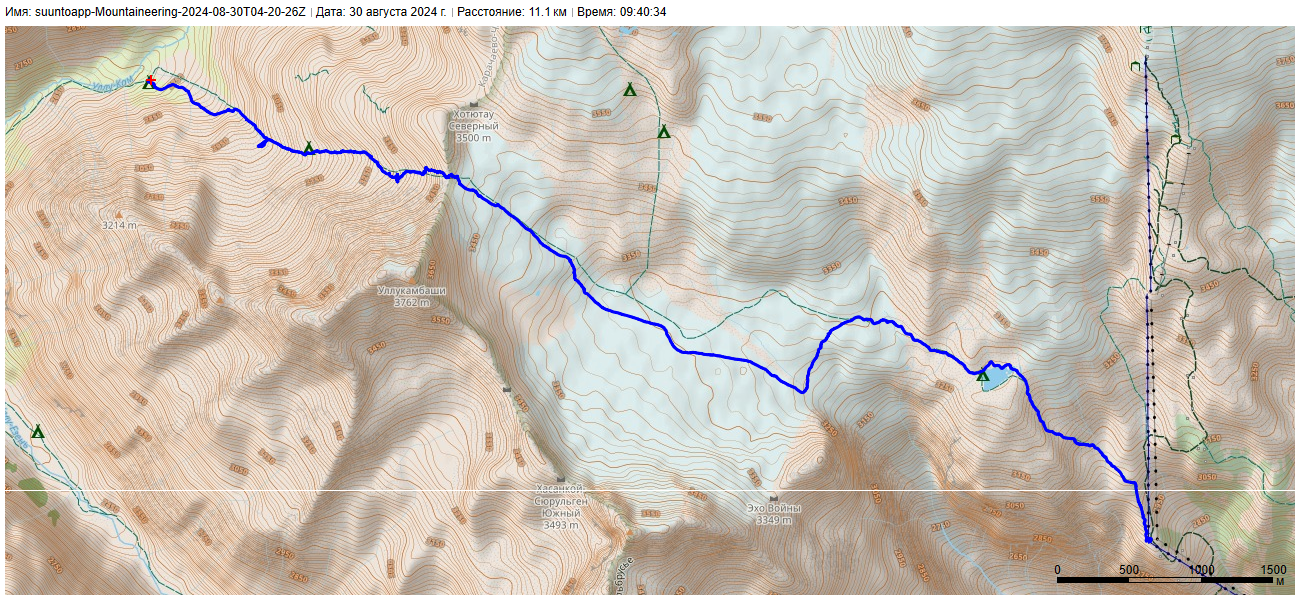
\includegraphics[angle=0, width=0.7\linewidth]{../pics/mini_maps/30}
	\label{fig:mini_30}
\end{figure}

Общий подъём в 05:30, выход в 07:20.

\begin{figure}[h!]
	\centering
	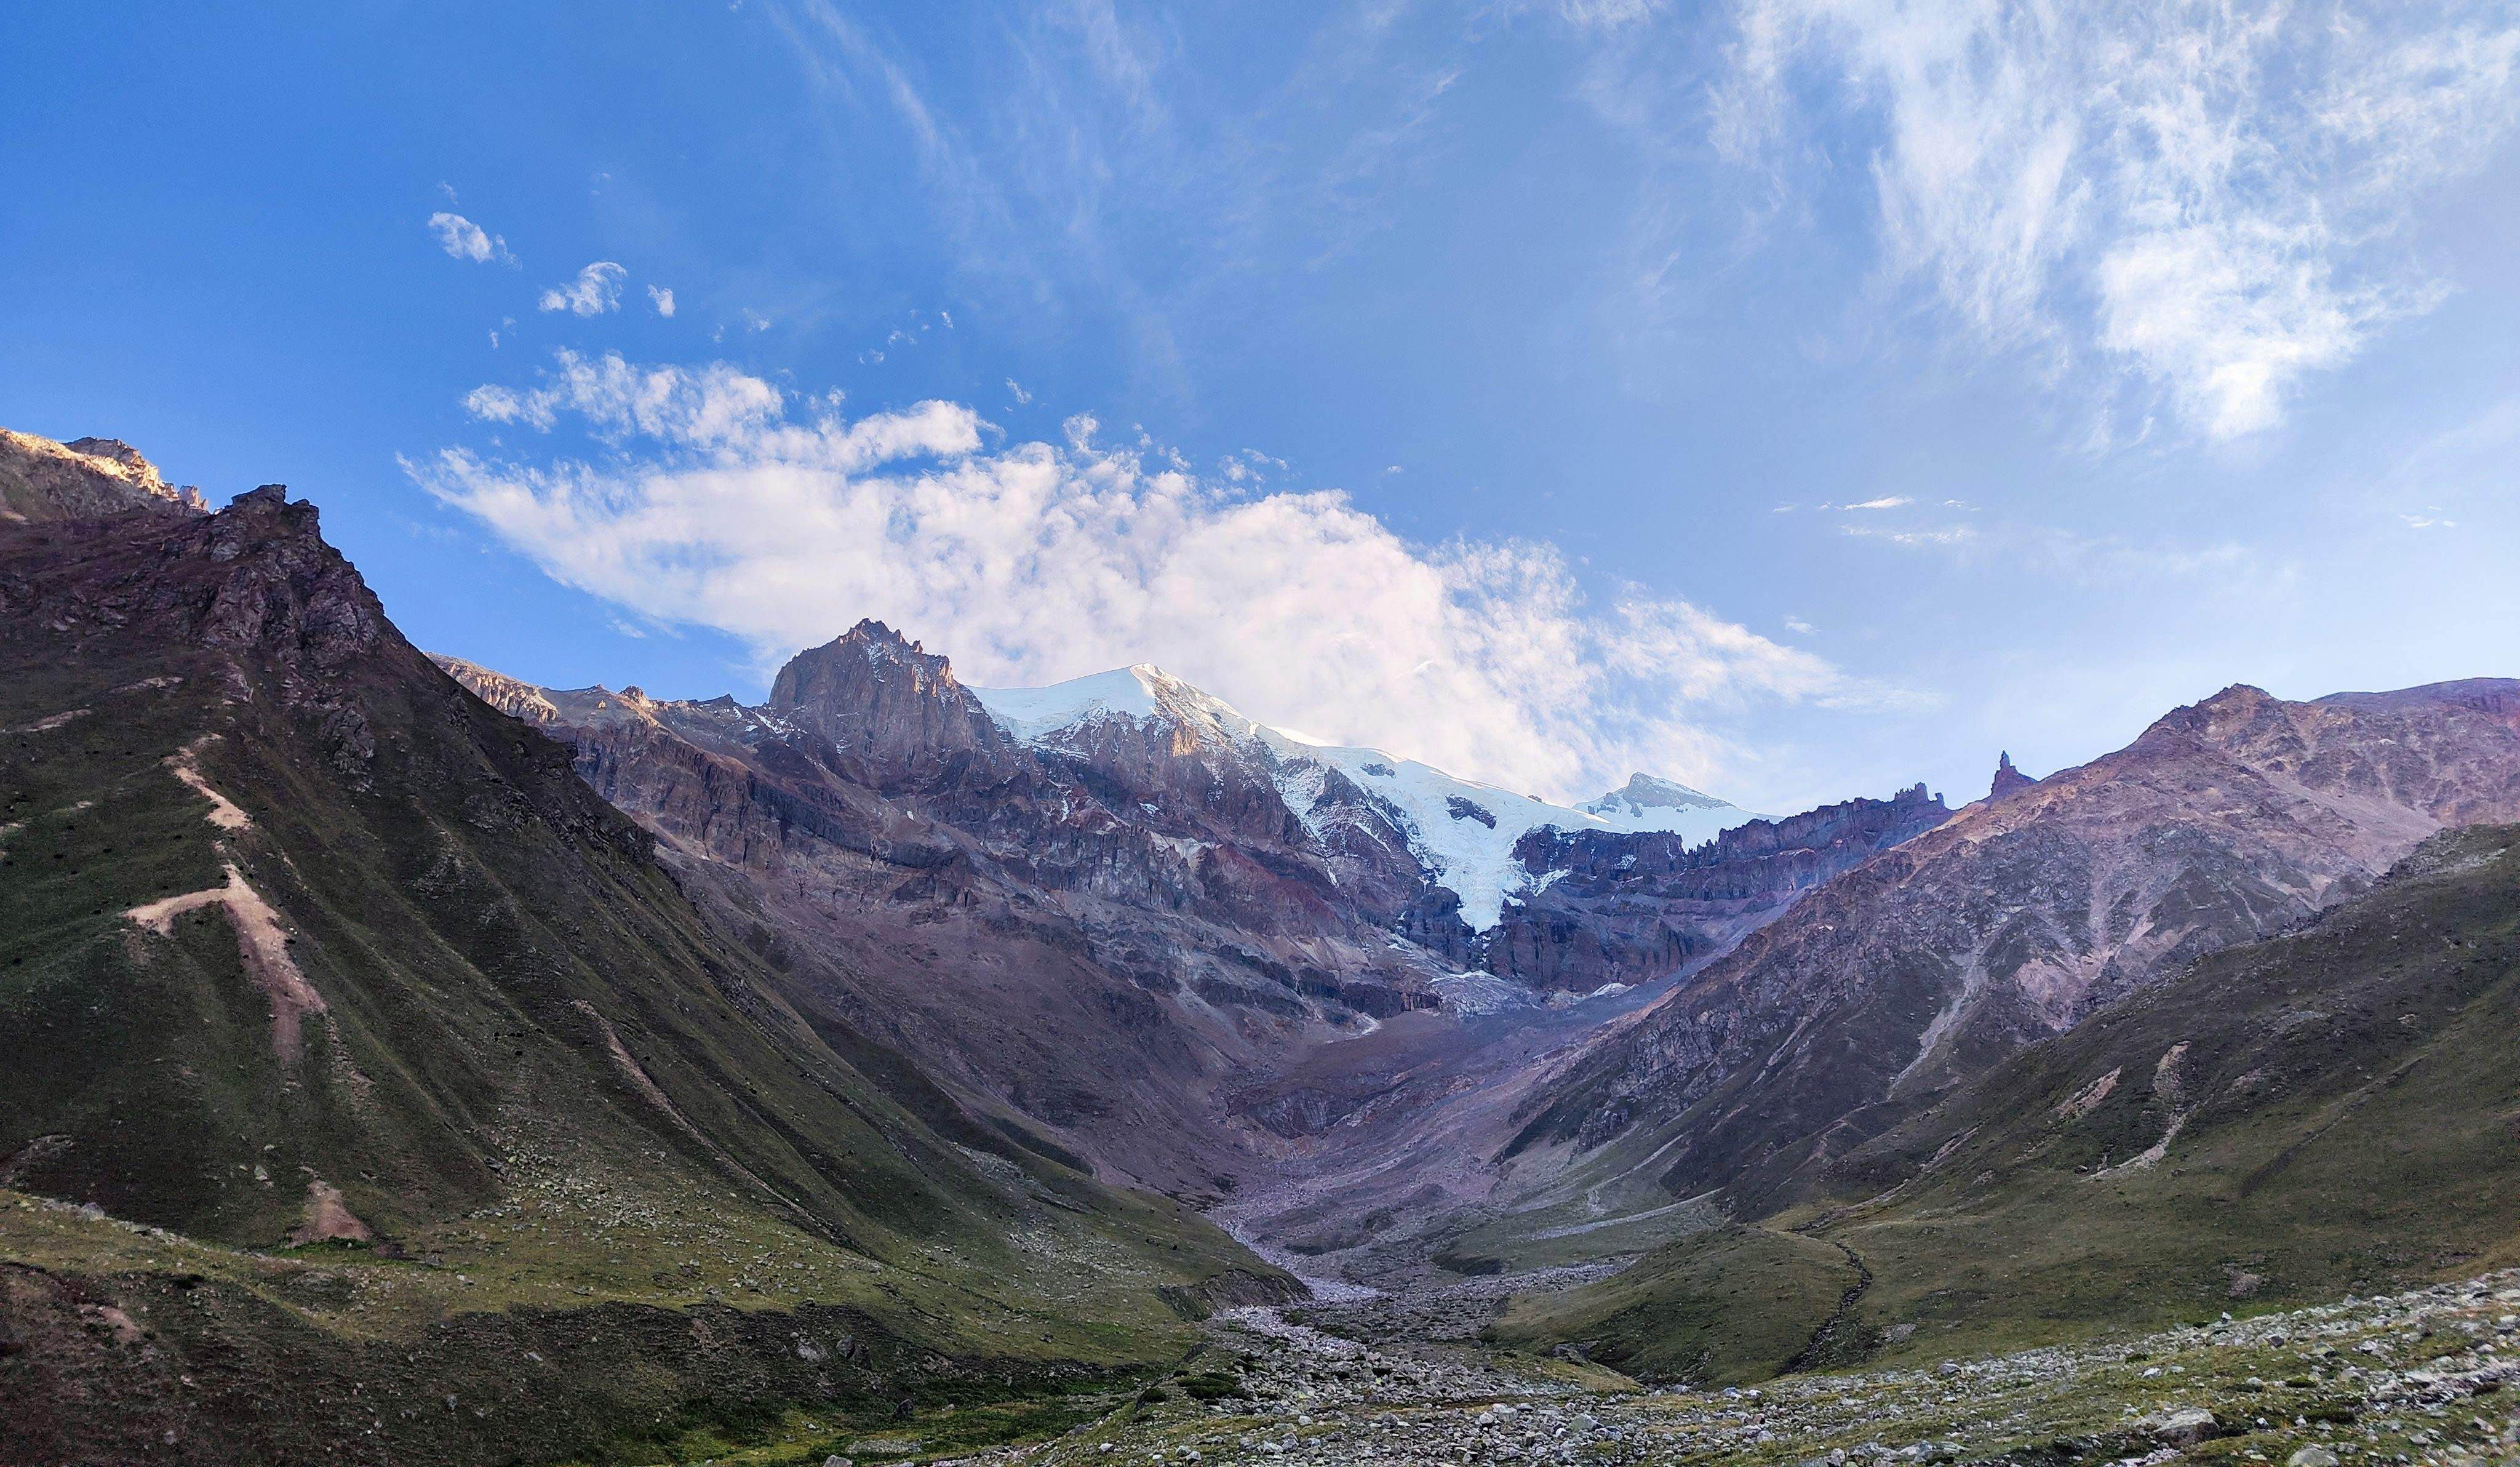
\includegraphics[width=0.7\linewidth]{../pics/IMG_20240830_063548}
	\caption{Утренний вид на юго-западные склоны Эльбруса}
	\label{fig:IMG_20240830_063548}
\end{figure}

До перевала ползли без особых проблем~--- сыпуха и курумник к концу похода стали нам родными и знакомыми. Путь технически и физически не сложный, но морально несколько утомляет, так как необходимо набрать 800 м высоты. Огромной поддержкой оказались синие метки трека для трейлраннеров Alpindustria Elbrus Race. Они значительно сократили нам время на поиск пути. Снег на перевальном взлёте отсутствует.

\begin{figure}[h!]
	\centering
	\begin{minipage}[h]{0.52\linewidth}
		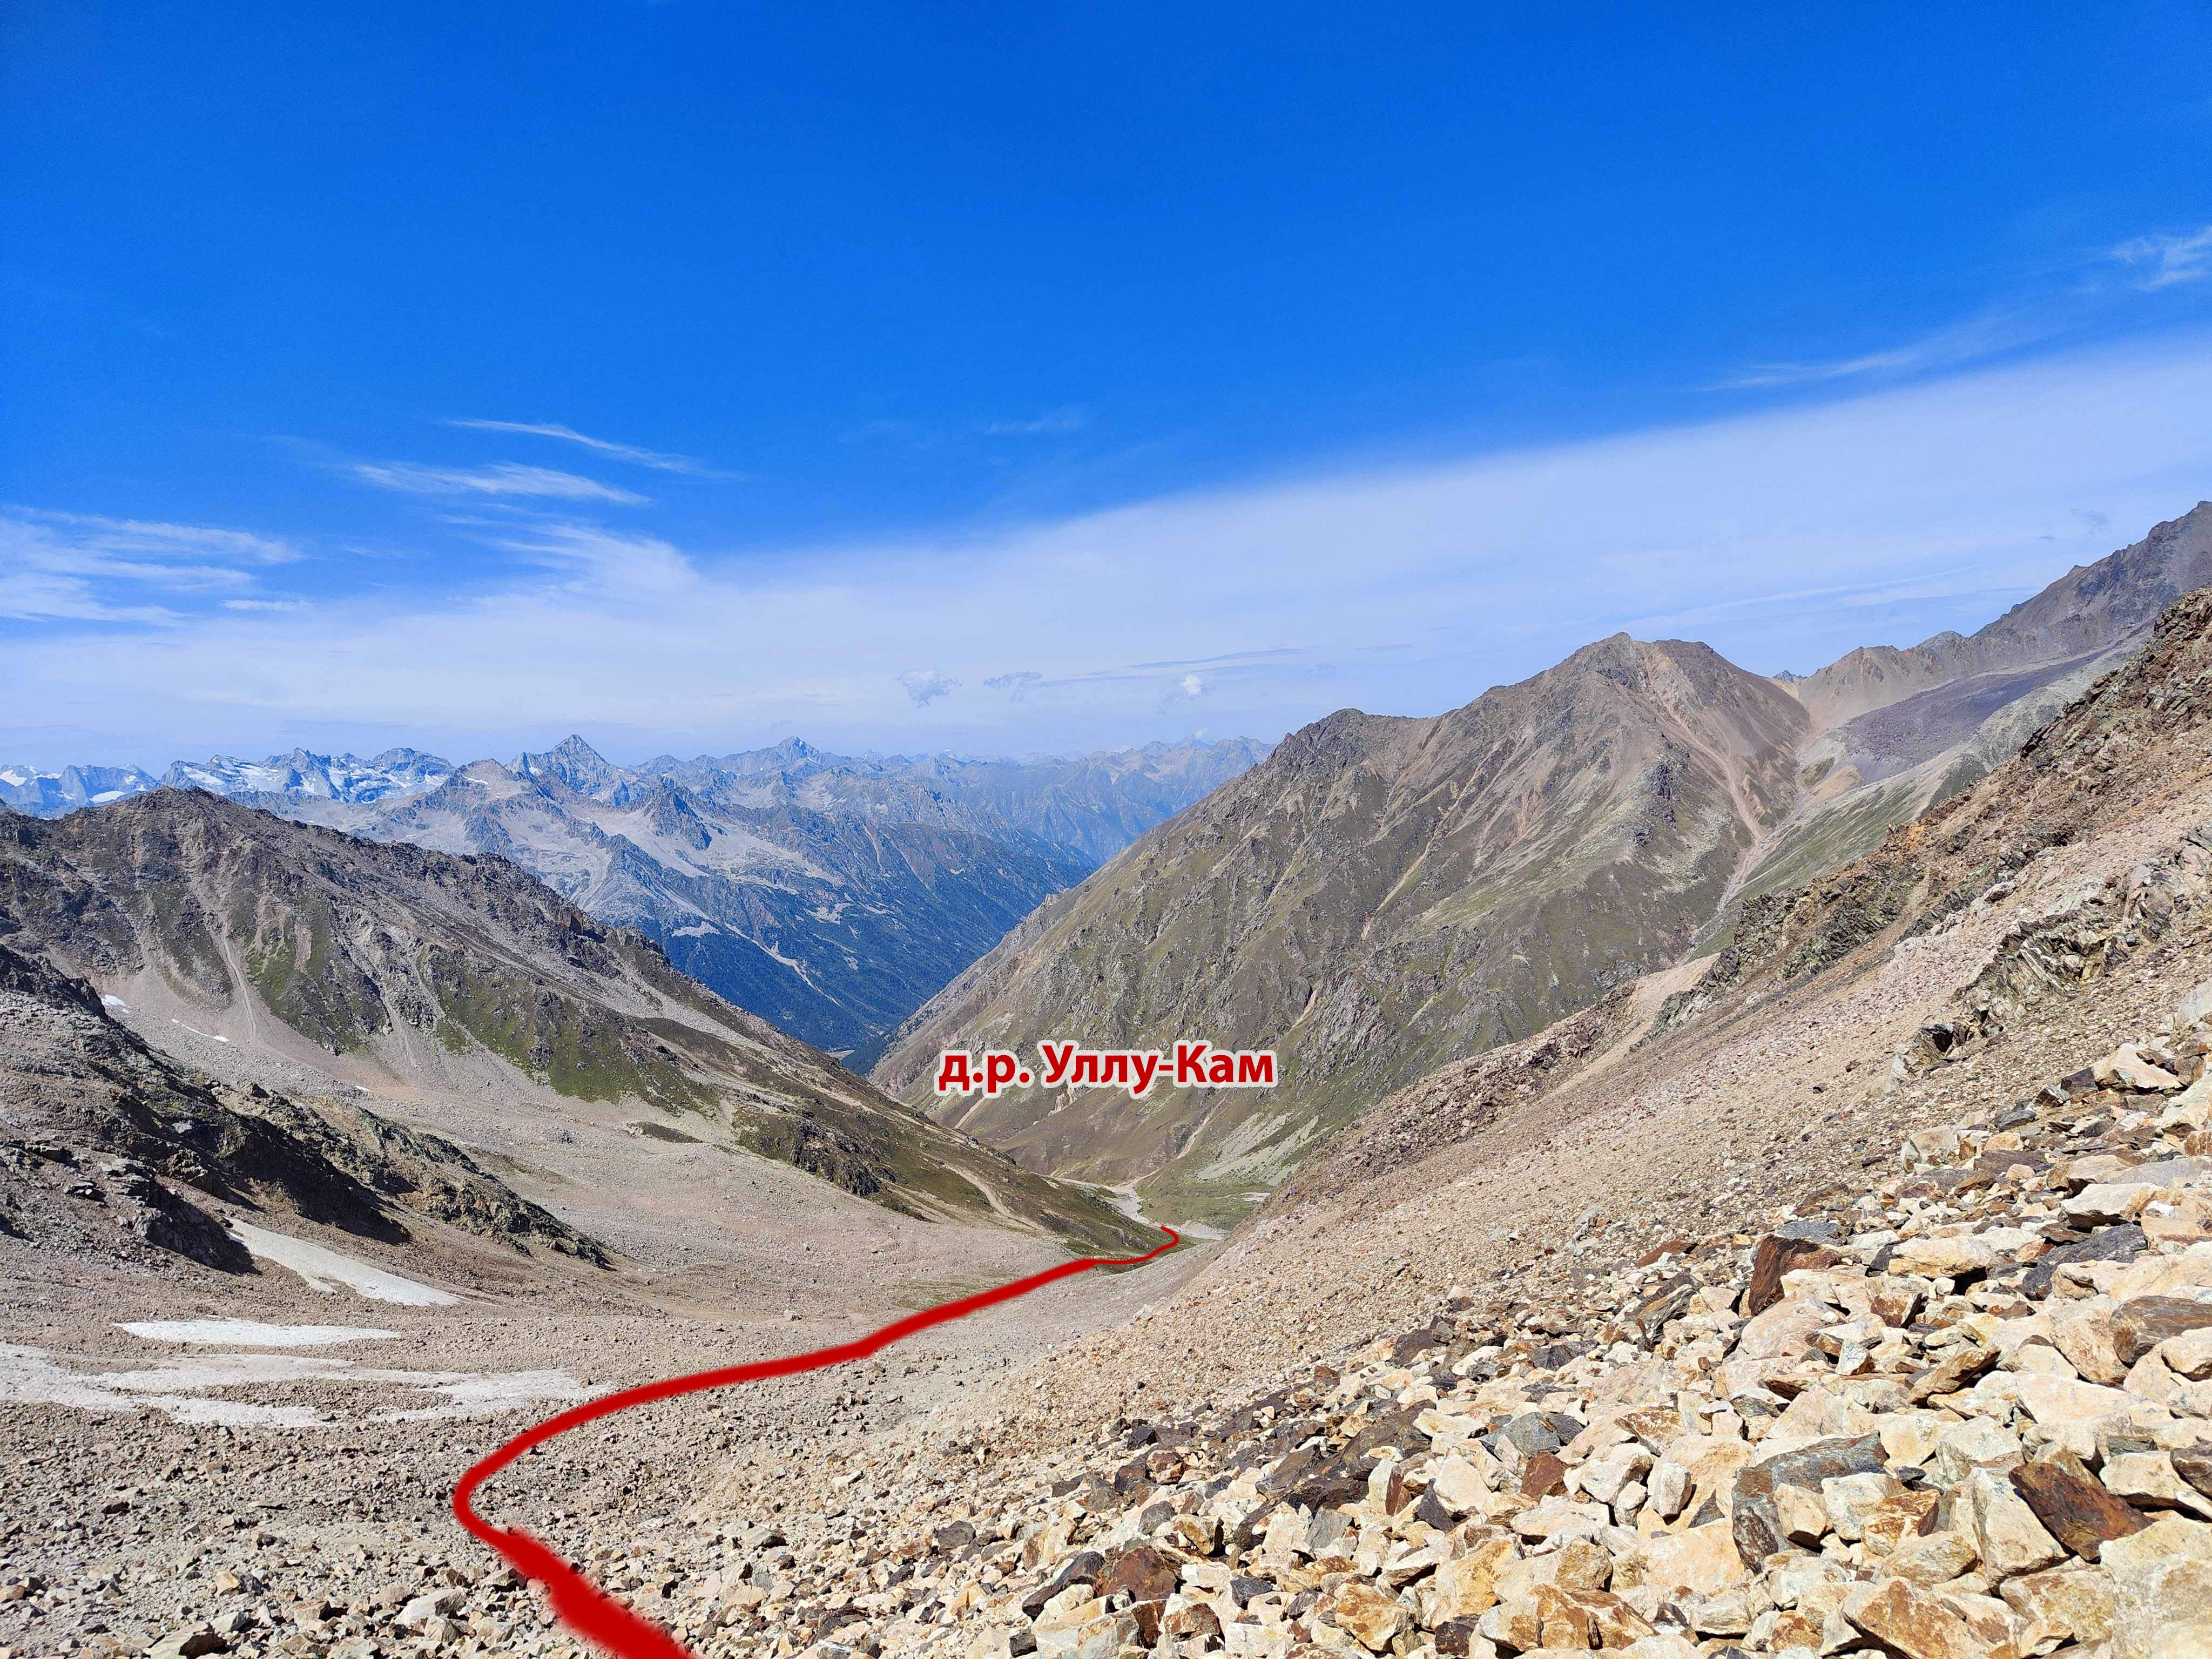
\includegraphics[width=0.99\linewidth]{../pics/IMG_20240830_105443}
	\end{minipage}
	\qquad
	\begin{minipage}[h]{0.29\linewidth}
		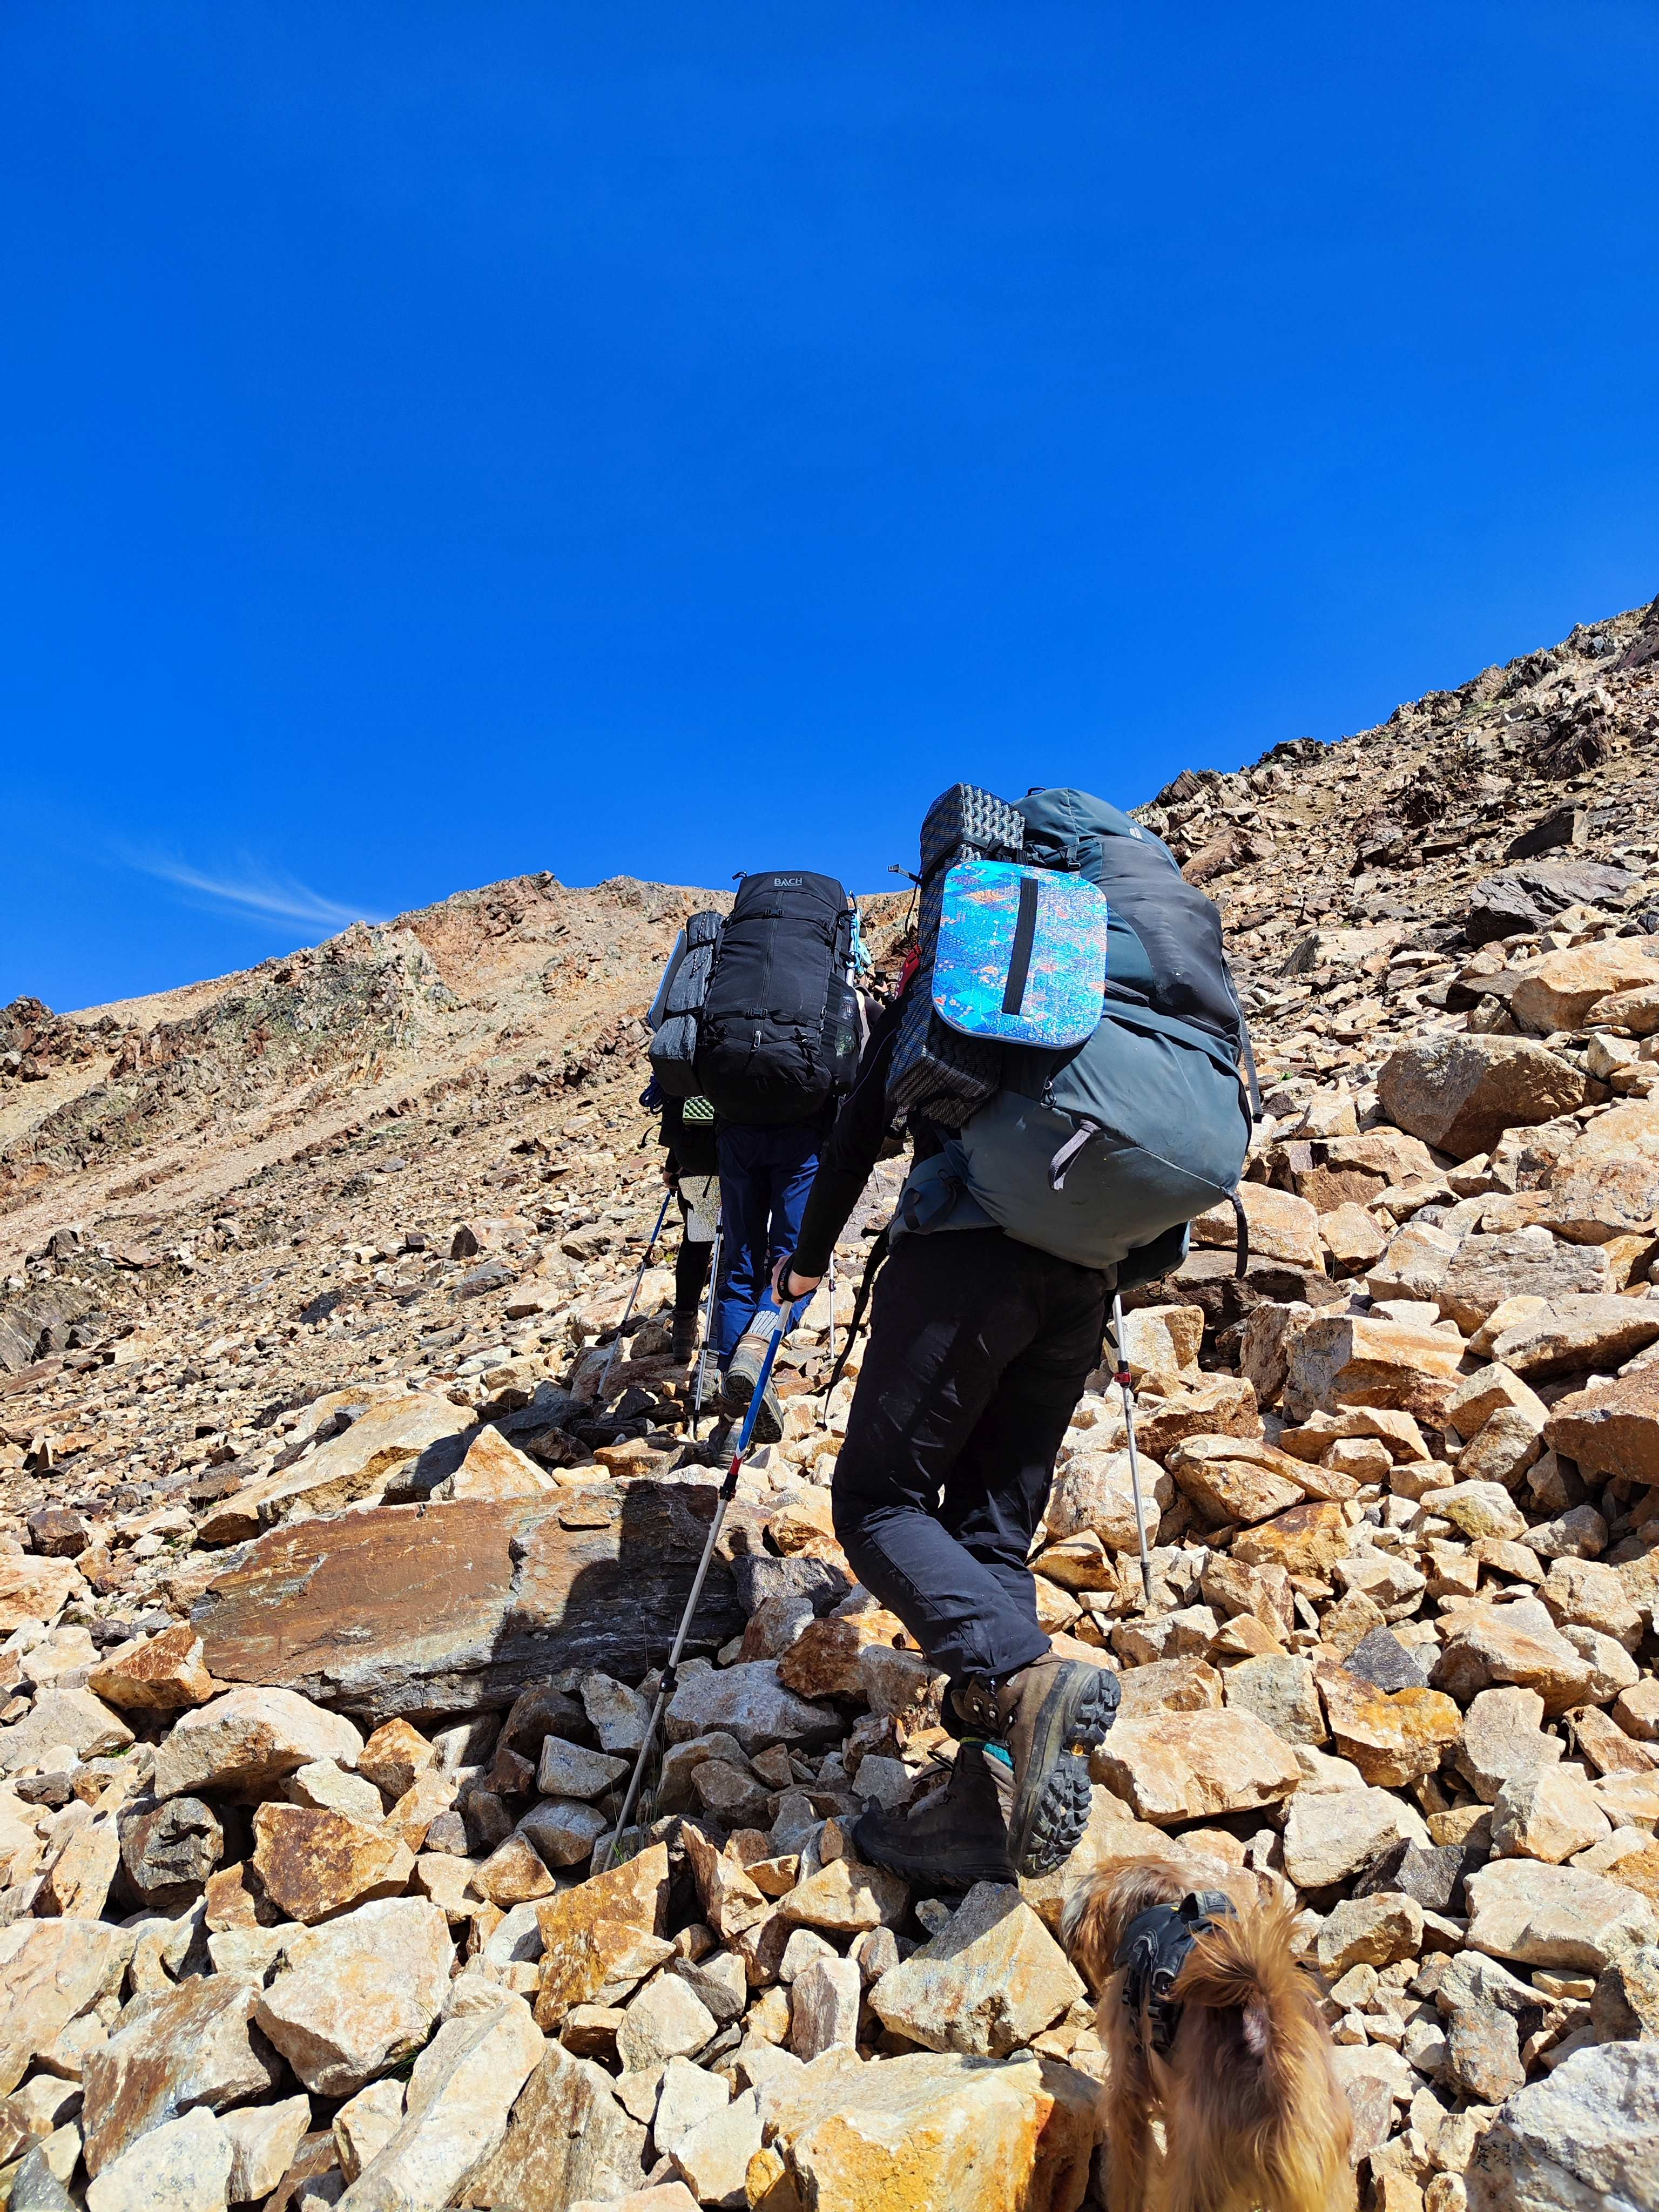
\includegraphics[width=0.99\linewidth]{../pics/IMG_20240830_105447}
	\end{minipage}
	\caption{Слева: вид на путь подъёма. Справа: поднимаемся на перевал}
	\label{fig:IMG_20240830_105443}
\end{figure}

В 11:30 поднялись на перевал. Погода, что для Хотютау нехарактерно, стояла шикарная, открывались потрясающие виды на горы Карачаево-Черкессии, Кабардино-Балкарии и, конечно, Эльбрус. Ледник Большой Азау, ожидаемо, был открыт. Отметили на перевале большое количество памятных табличек, посвящённых военным действиям в годы ВОВ. Сфотографировались, отзвонились и отписались родным, порадовались малому количеству мусора на перевале (судя по отчётам~\cite{Korolyov2018}, с этим были проблемы). Сняли сразу две перевальные записки: проекта <<Виртуальные горы>> от 28.08.2024 и турклуба <<ЛИИЖТ>> г. Санкт-Петербург от 21.08.2024.

\begin{figure}[h!]
	\centering
	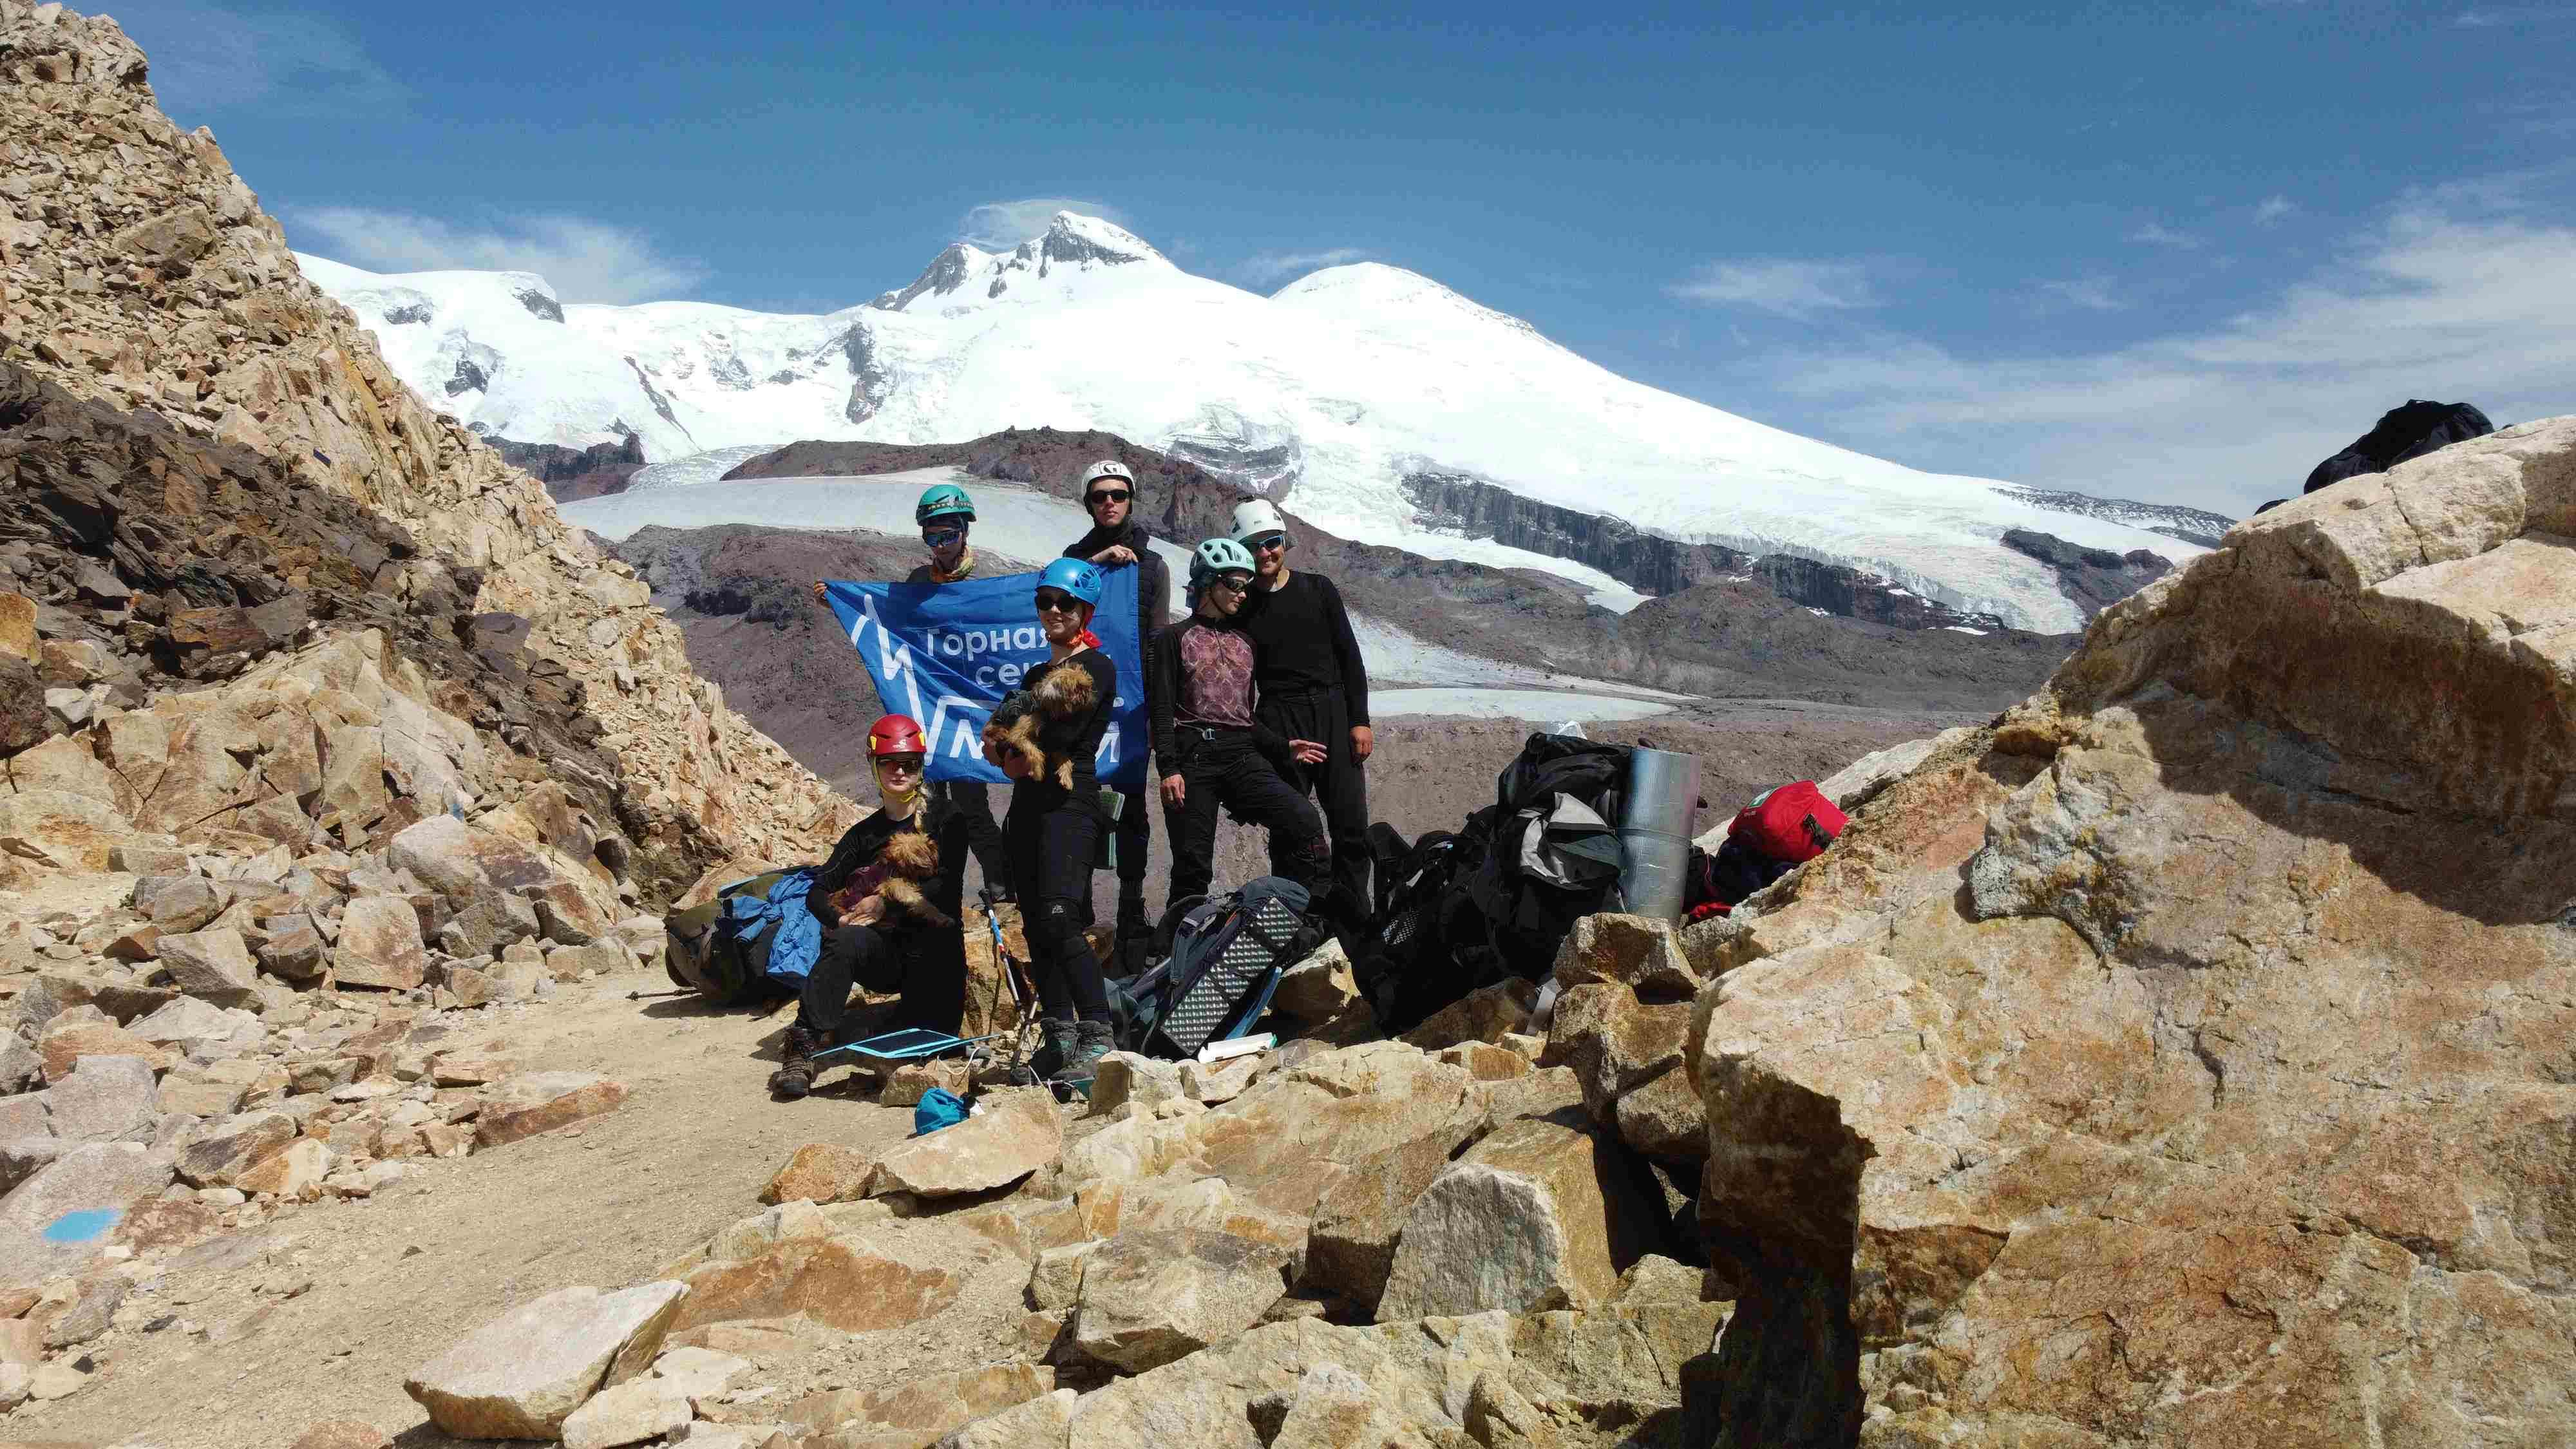
\includegraphics[width=0.7\linewidth]{../pics/DJI_0899}
	\caption{группа на пер. Хотютау}
	\label{fig:hotyutau_1}
\end{figure}

В 12:30 начали спуск. На ледник спуск шёл по мелкой сыпухе, в связи с чем руководитель и замруководителя пытались показать группе спуск <<лифтом>>. В 12:49 вышли на ледник. Заметили на седловине перевала двух туристов, надели кошки и начали движение по леднику. Поскольку ледник был открытый, трещины хорошо просматривались и легко обходились; но на всякий случай каждый участник опоясался куском блокировки и держал при себе два карабина и жумар.

\begin{figure}[h!]
	\centering
	\begin{minipage}[h]{0.4\linewidth}
		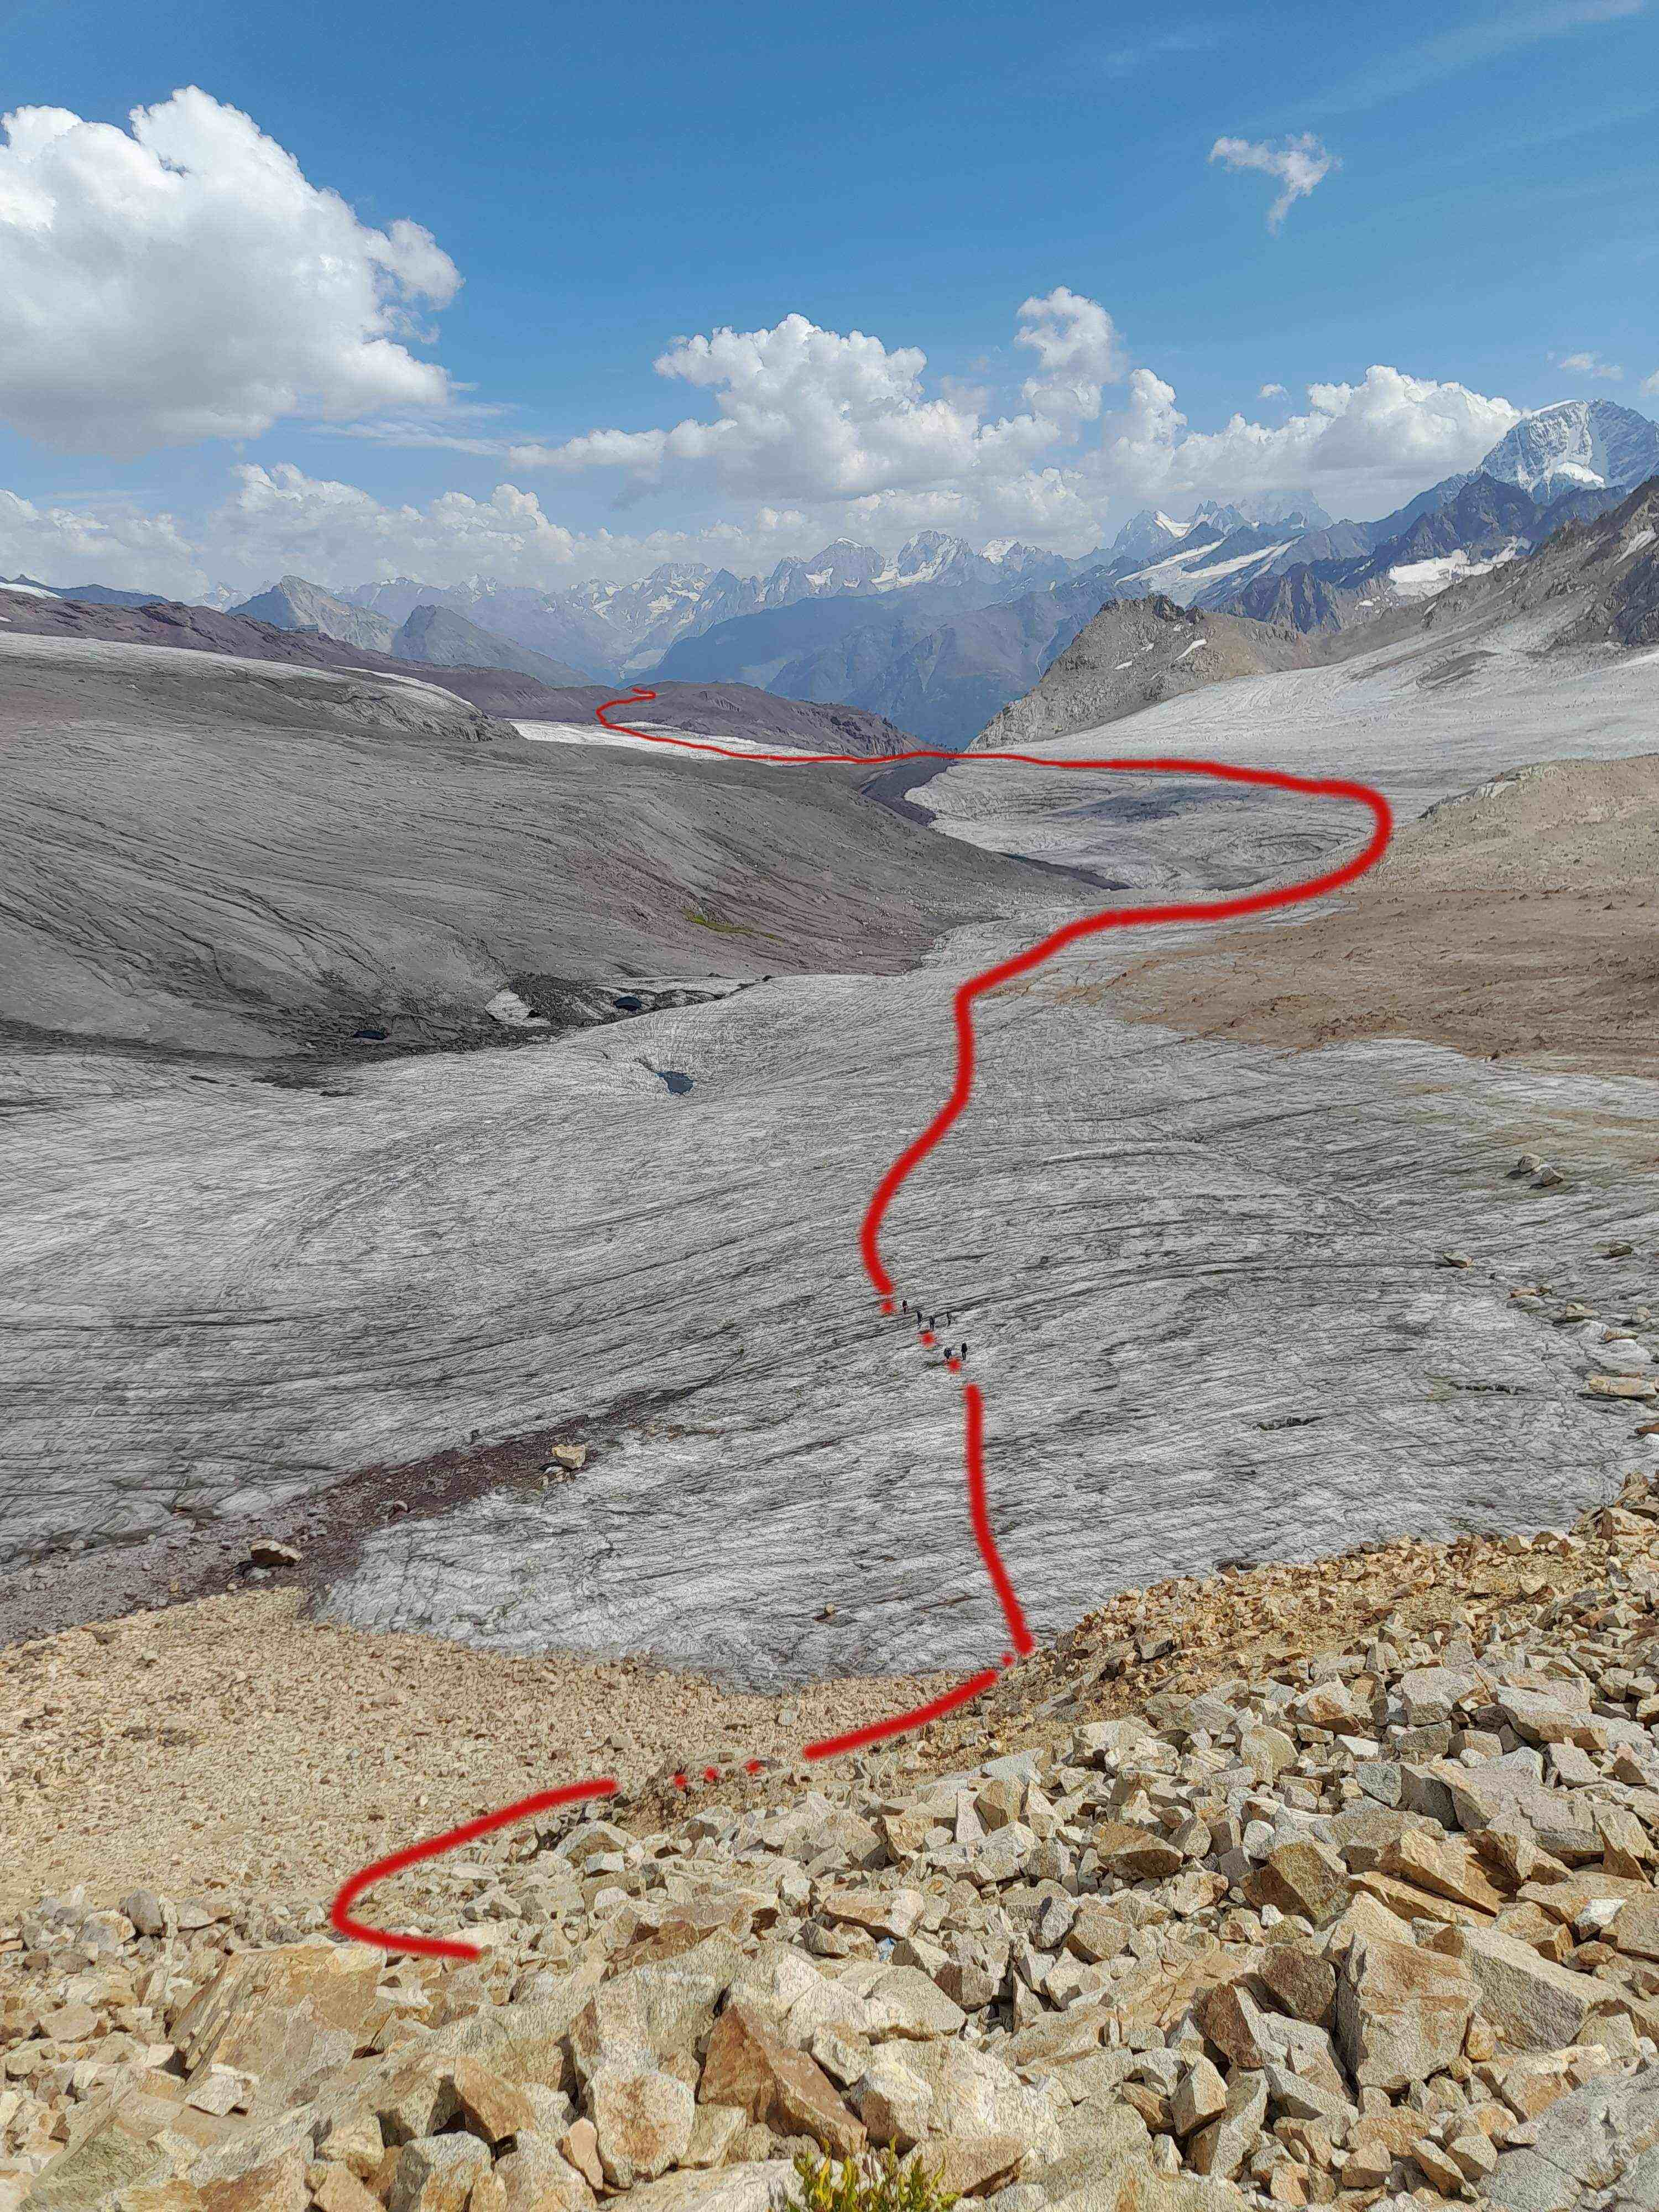
\includegraphics[width=0.99\linewidth]{../pics/20240830_141852.jpg}
	\end{minipage}
	\qquad
	\begin{minipage}[h]{0.4\linewidth}
		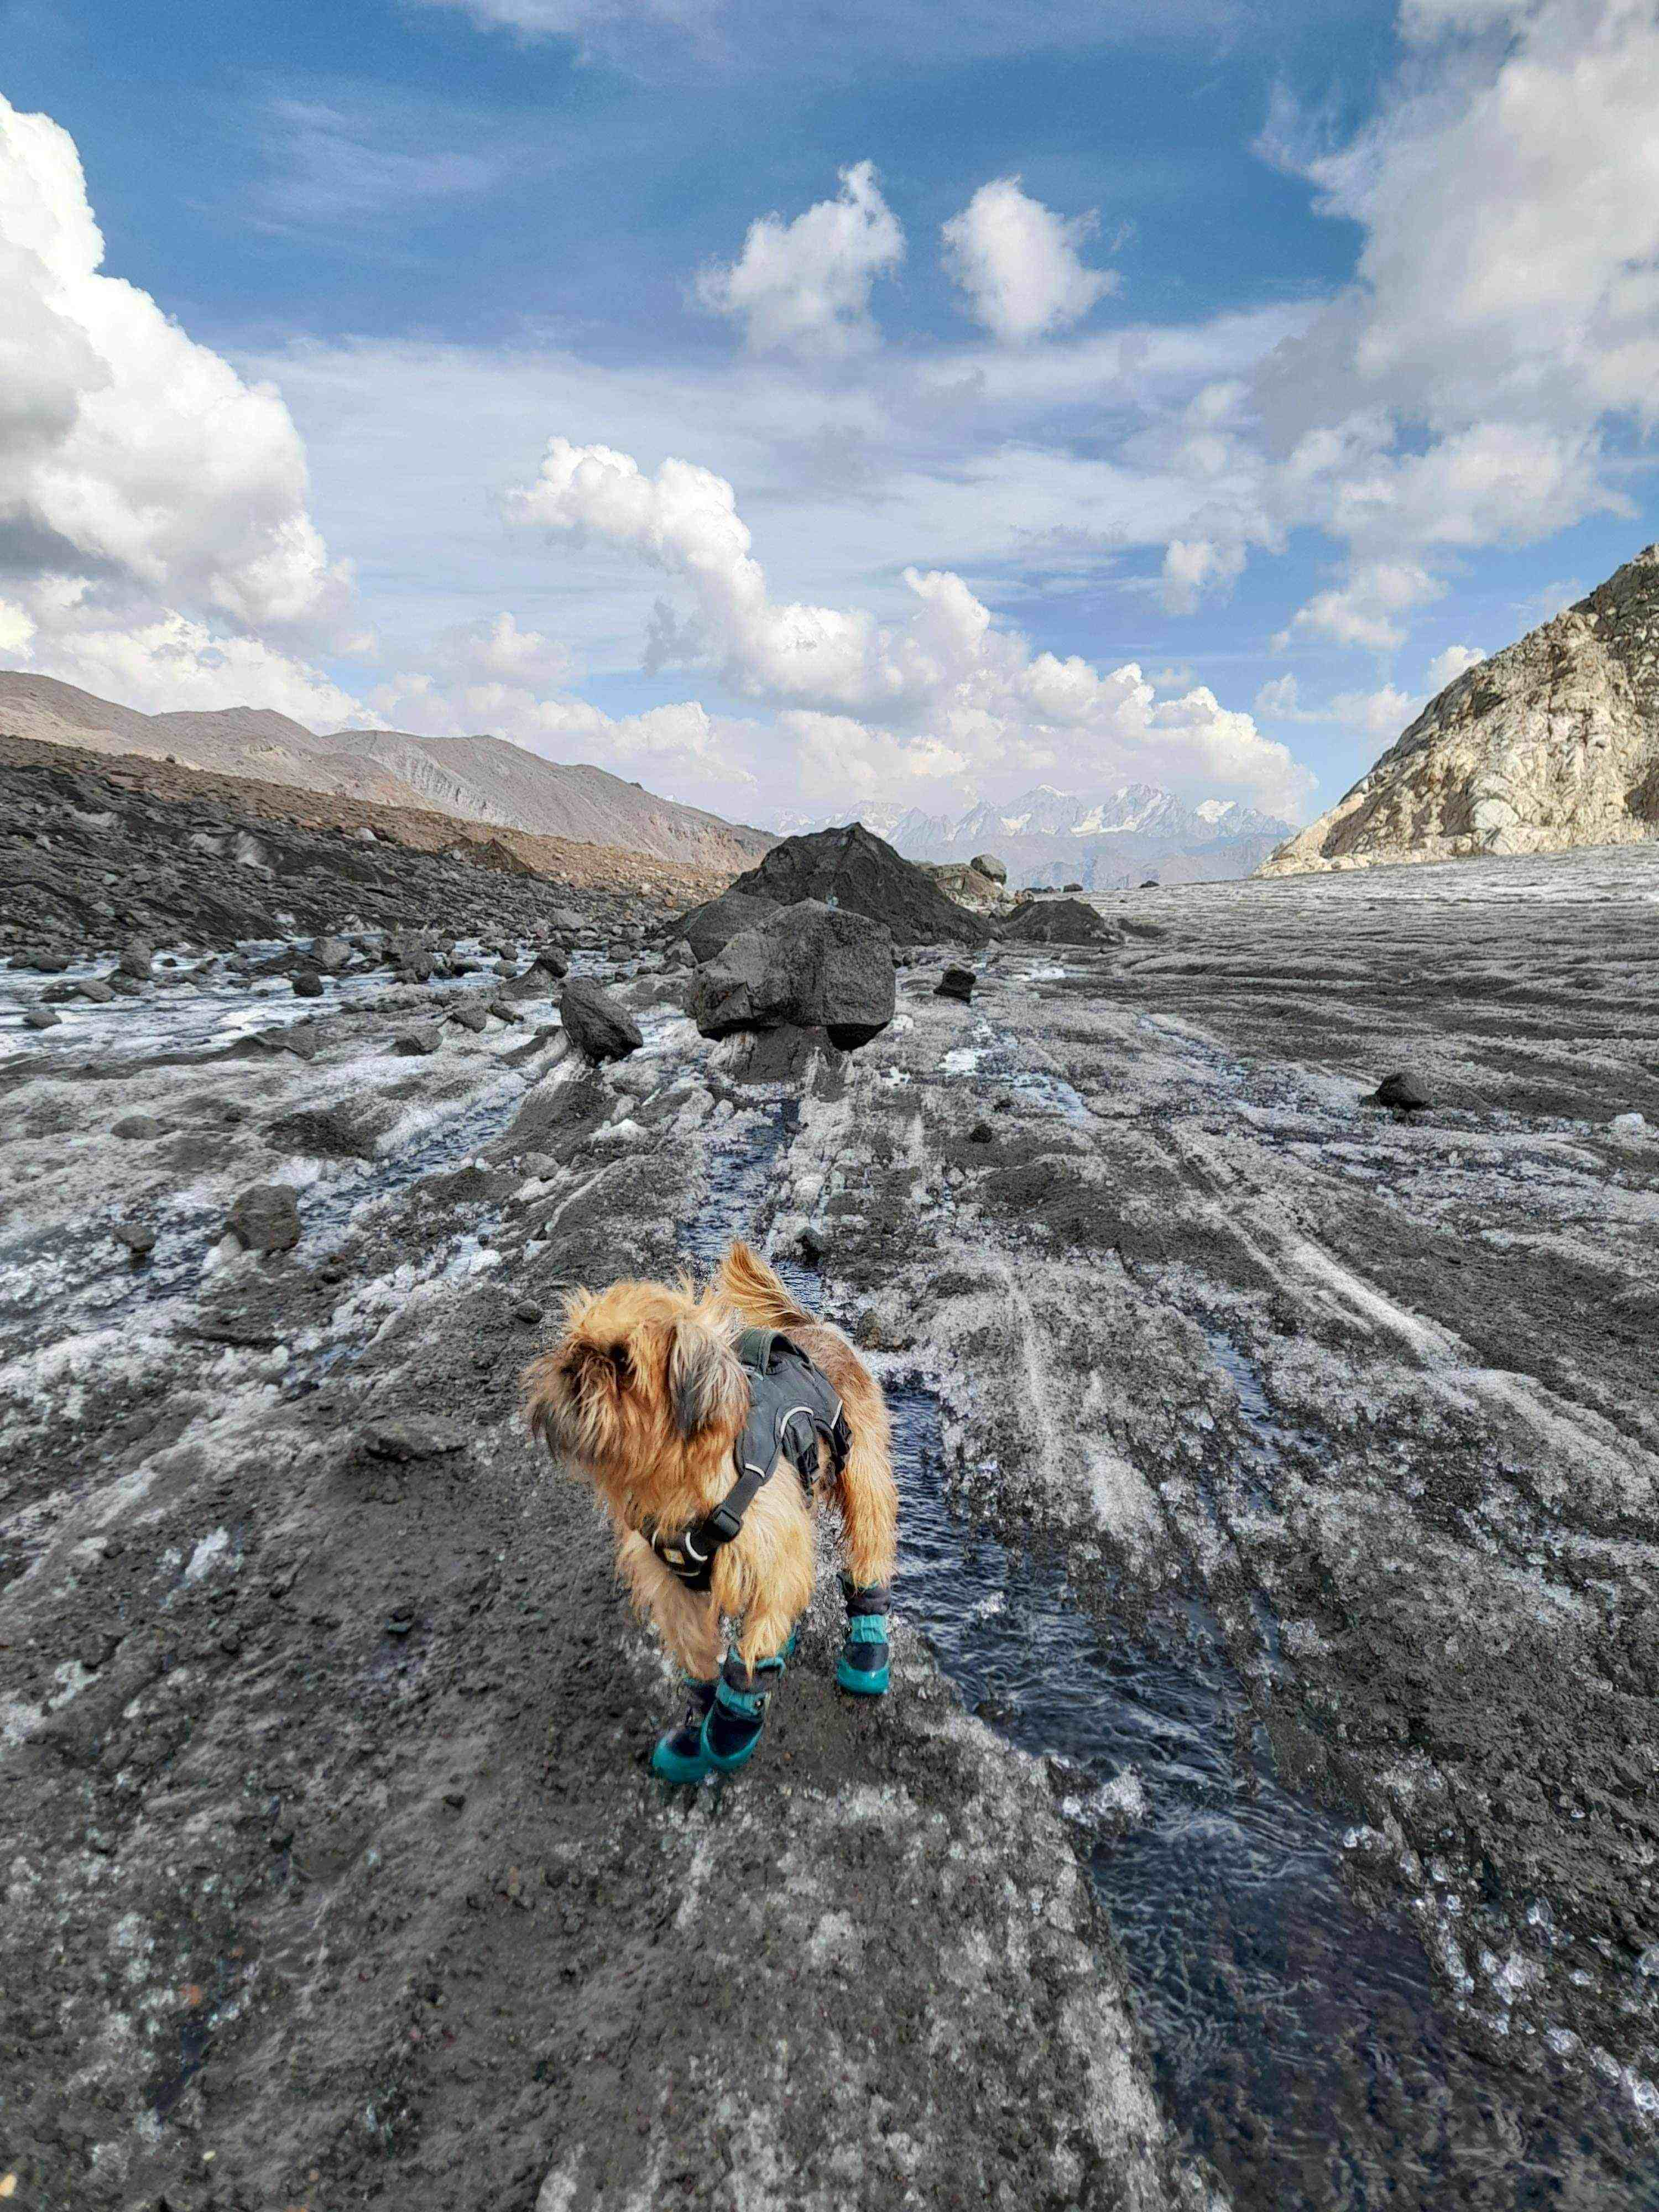
\includegraphics[width=0.99\linewidth]{../pics/20240830_155136.jpg}
	\end{minipage}
	\caption{Слева: группа на леднике. Фото туристов т/к МАИ. Справа: единственный раз, когда собакам действительно пригодились ботинки~--- это переход по леднику}
	\label{fig:20240830_141852}
\end{figure}

На ближайшем привале нас догнали туристы горной секции МАИ. Как выяснилось, оставленная нами записка пролежала в камнях не более получаса. Увеличенным составом мы продолжили движение по леднику и таки допустили досадную ошибку, пройдя мимо нужного участка <<красной>> и <<чёрной>> морен и не свернув вовремя налево пхд. В конце концов ошибку исправили и повернули в нужную сторону в 15:00 --- но из-за этого пришлось набирать лишние 50~м высоты. На ледовые поля тем временем стал спускаться плотный туман, поэтому мы были очень рады, когда, наконец, увидели на моренах знакомую синюю метку. По хорошо протоптанной дорожке далее шли без проблем. 

В 16:20 вышли к Эльбрусскому озеру. Руководитель принял решение обойти его с севера, хотя стоит заметить, что трейлраннинговая тропа идёт по противоположному, южному берегу.

\begin{figure}[h!]
	\centering
	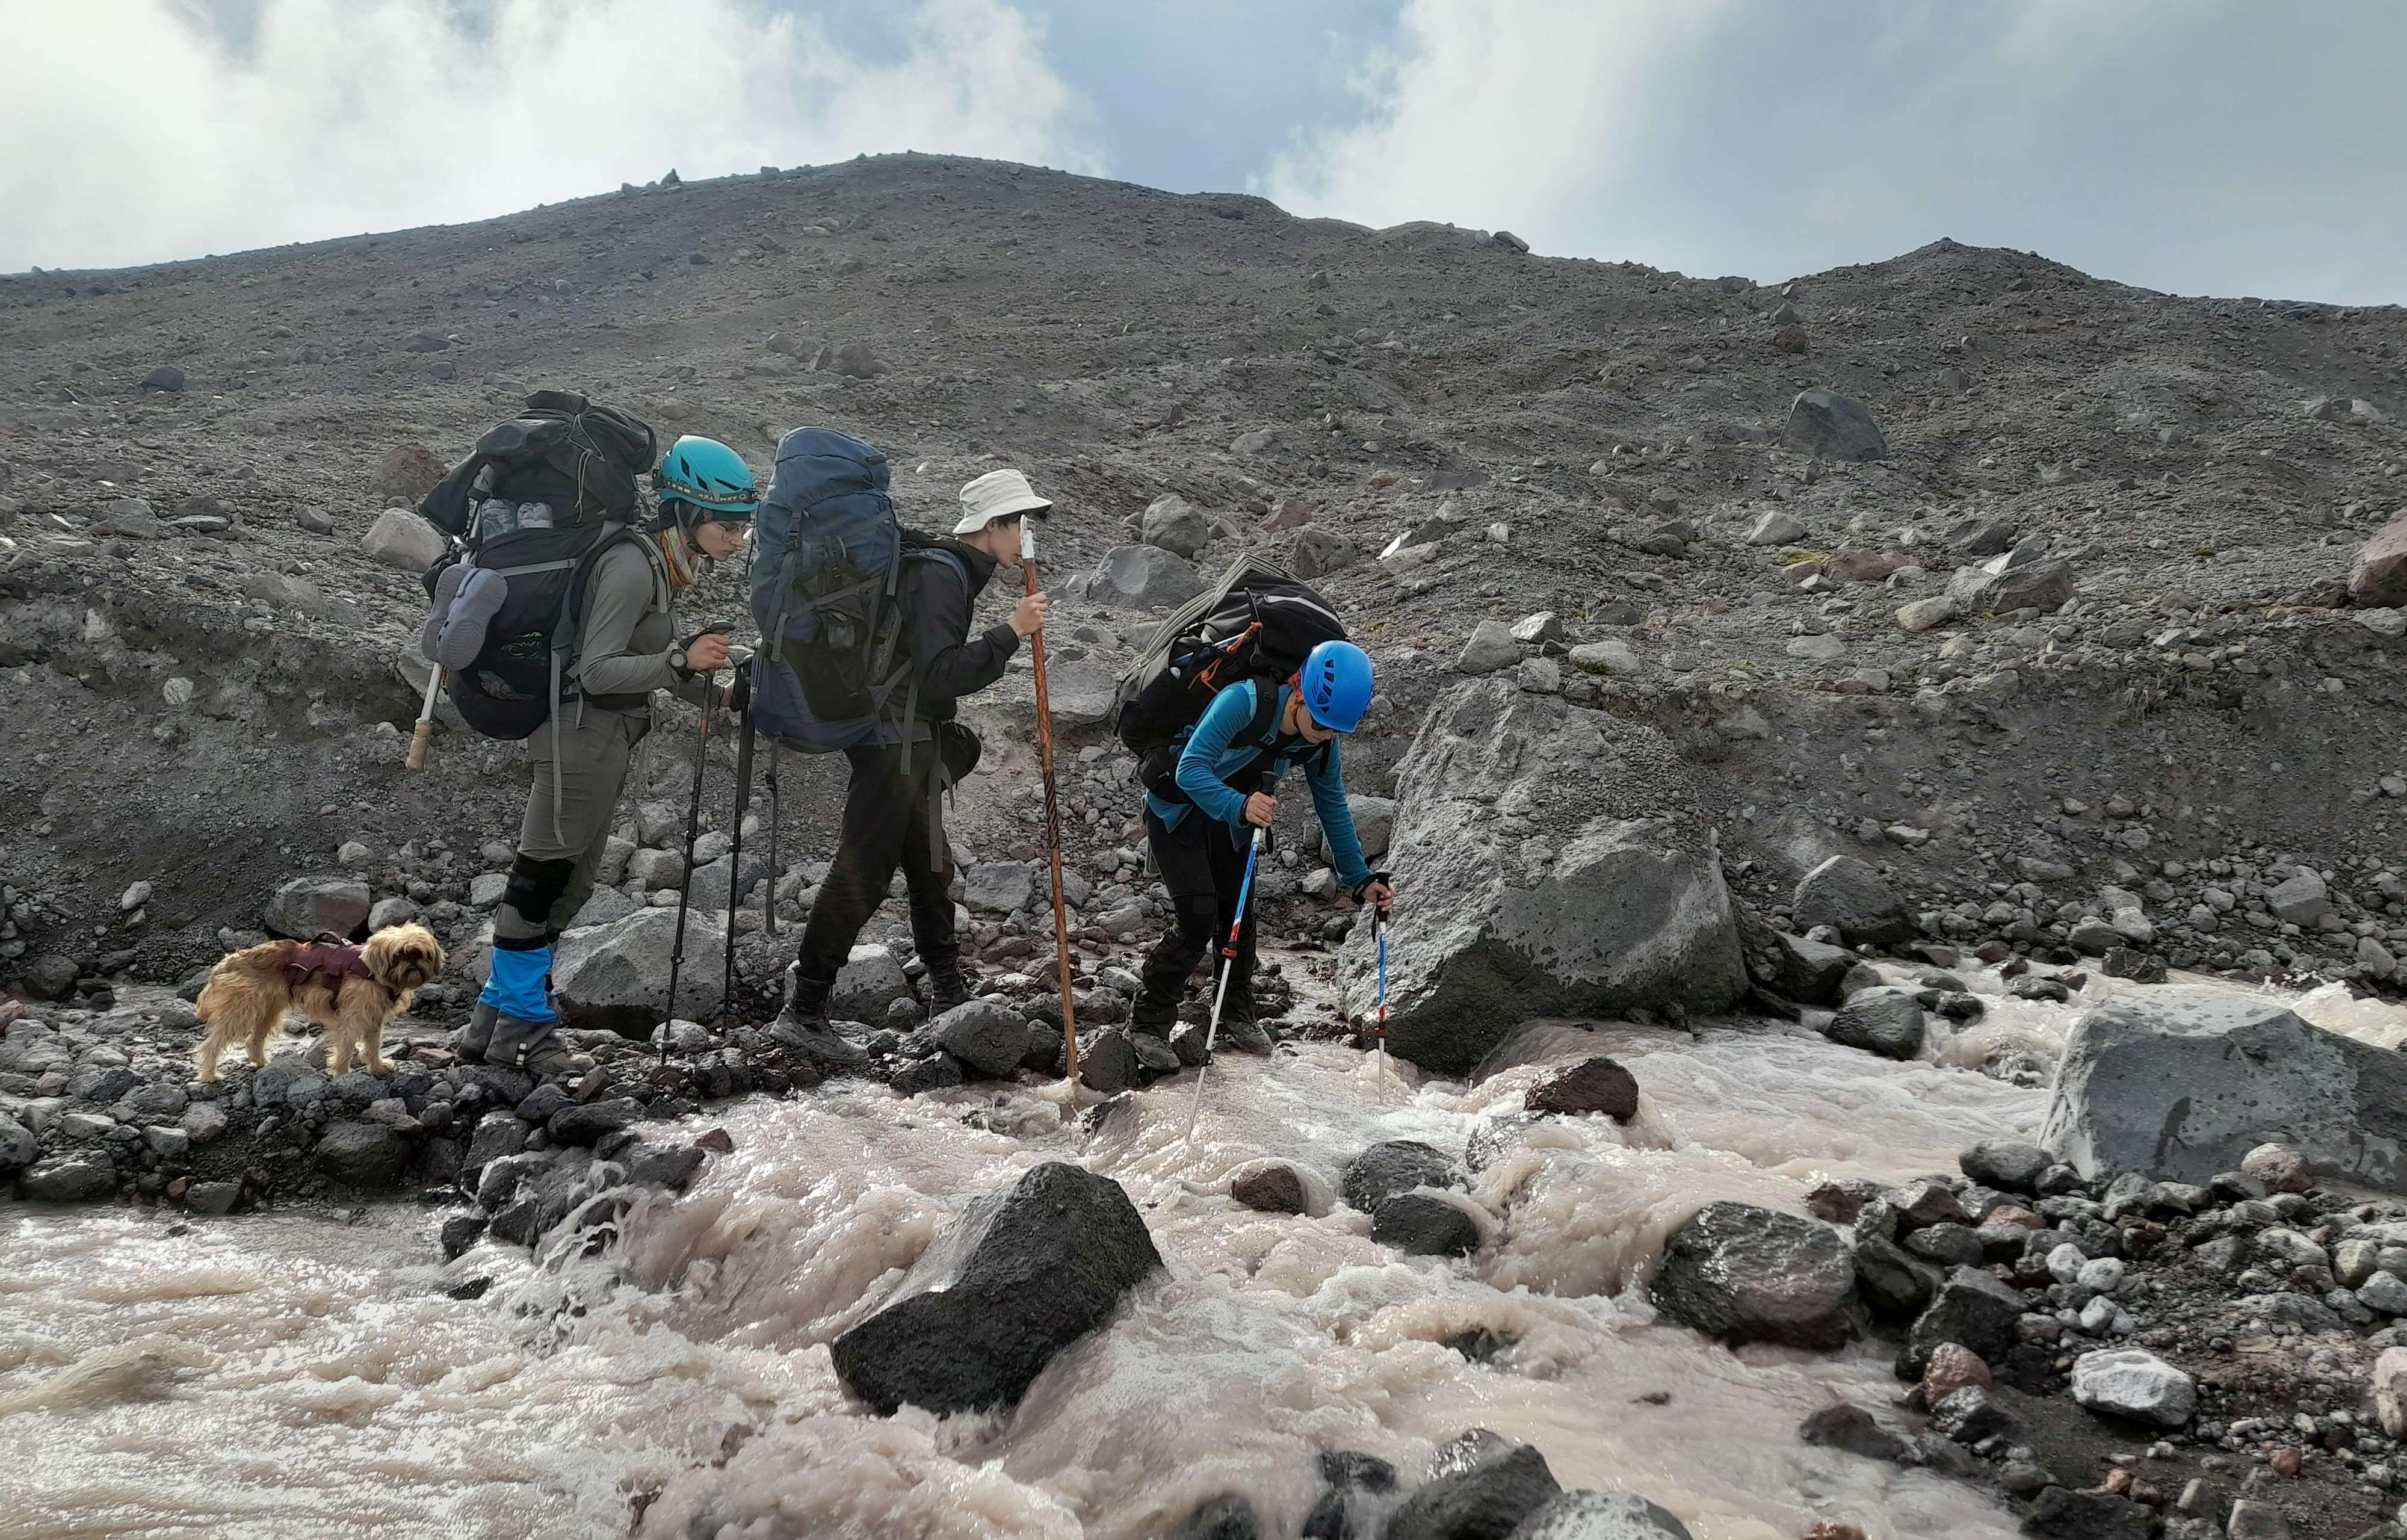
\includegraphics[width=0.7\linewidth]{../pics/20240830_162252.jpg}
	\caption{Бродим ручей, впадающий в Эльбрусское озеро}
	\label{fig:20240830_162252.jpg}
\end{figure}

В этот момент выяснилось, что до закрытия канатной дороги осталось меньше получаса: новая канатная дорога работает на спуск до 17:00. Остаток пути от озера до станции <<Кругозор>> представляет собой довольно крутой спуск. Сейчас он безопасен и хорошо оборудован, ибо, помимо протоптанной тропы и синей маркировки, имеются оборудованные мосты через ручьи и виа-ферраты на локальных крутых участках. Шли на всех пар\'{а}х, изображая из себя трейлраннеров с рюкзаками за плечами: за 25 минут пробежали 2 км со сбросом 310 м. Передовая группа, состоящая из руководителя (Даши), Кати и Димы Дёмушкина, добежала до станции канатной дороги ровно в 17:00 и умоляла смотрителя разрешить нашей группе спуститься. Забег оказался не напрасным, и вся группа благополучно села на канатную дорогу ровно в 17:00. 

\begin{figure}[h!]
	\centering
	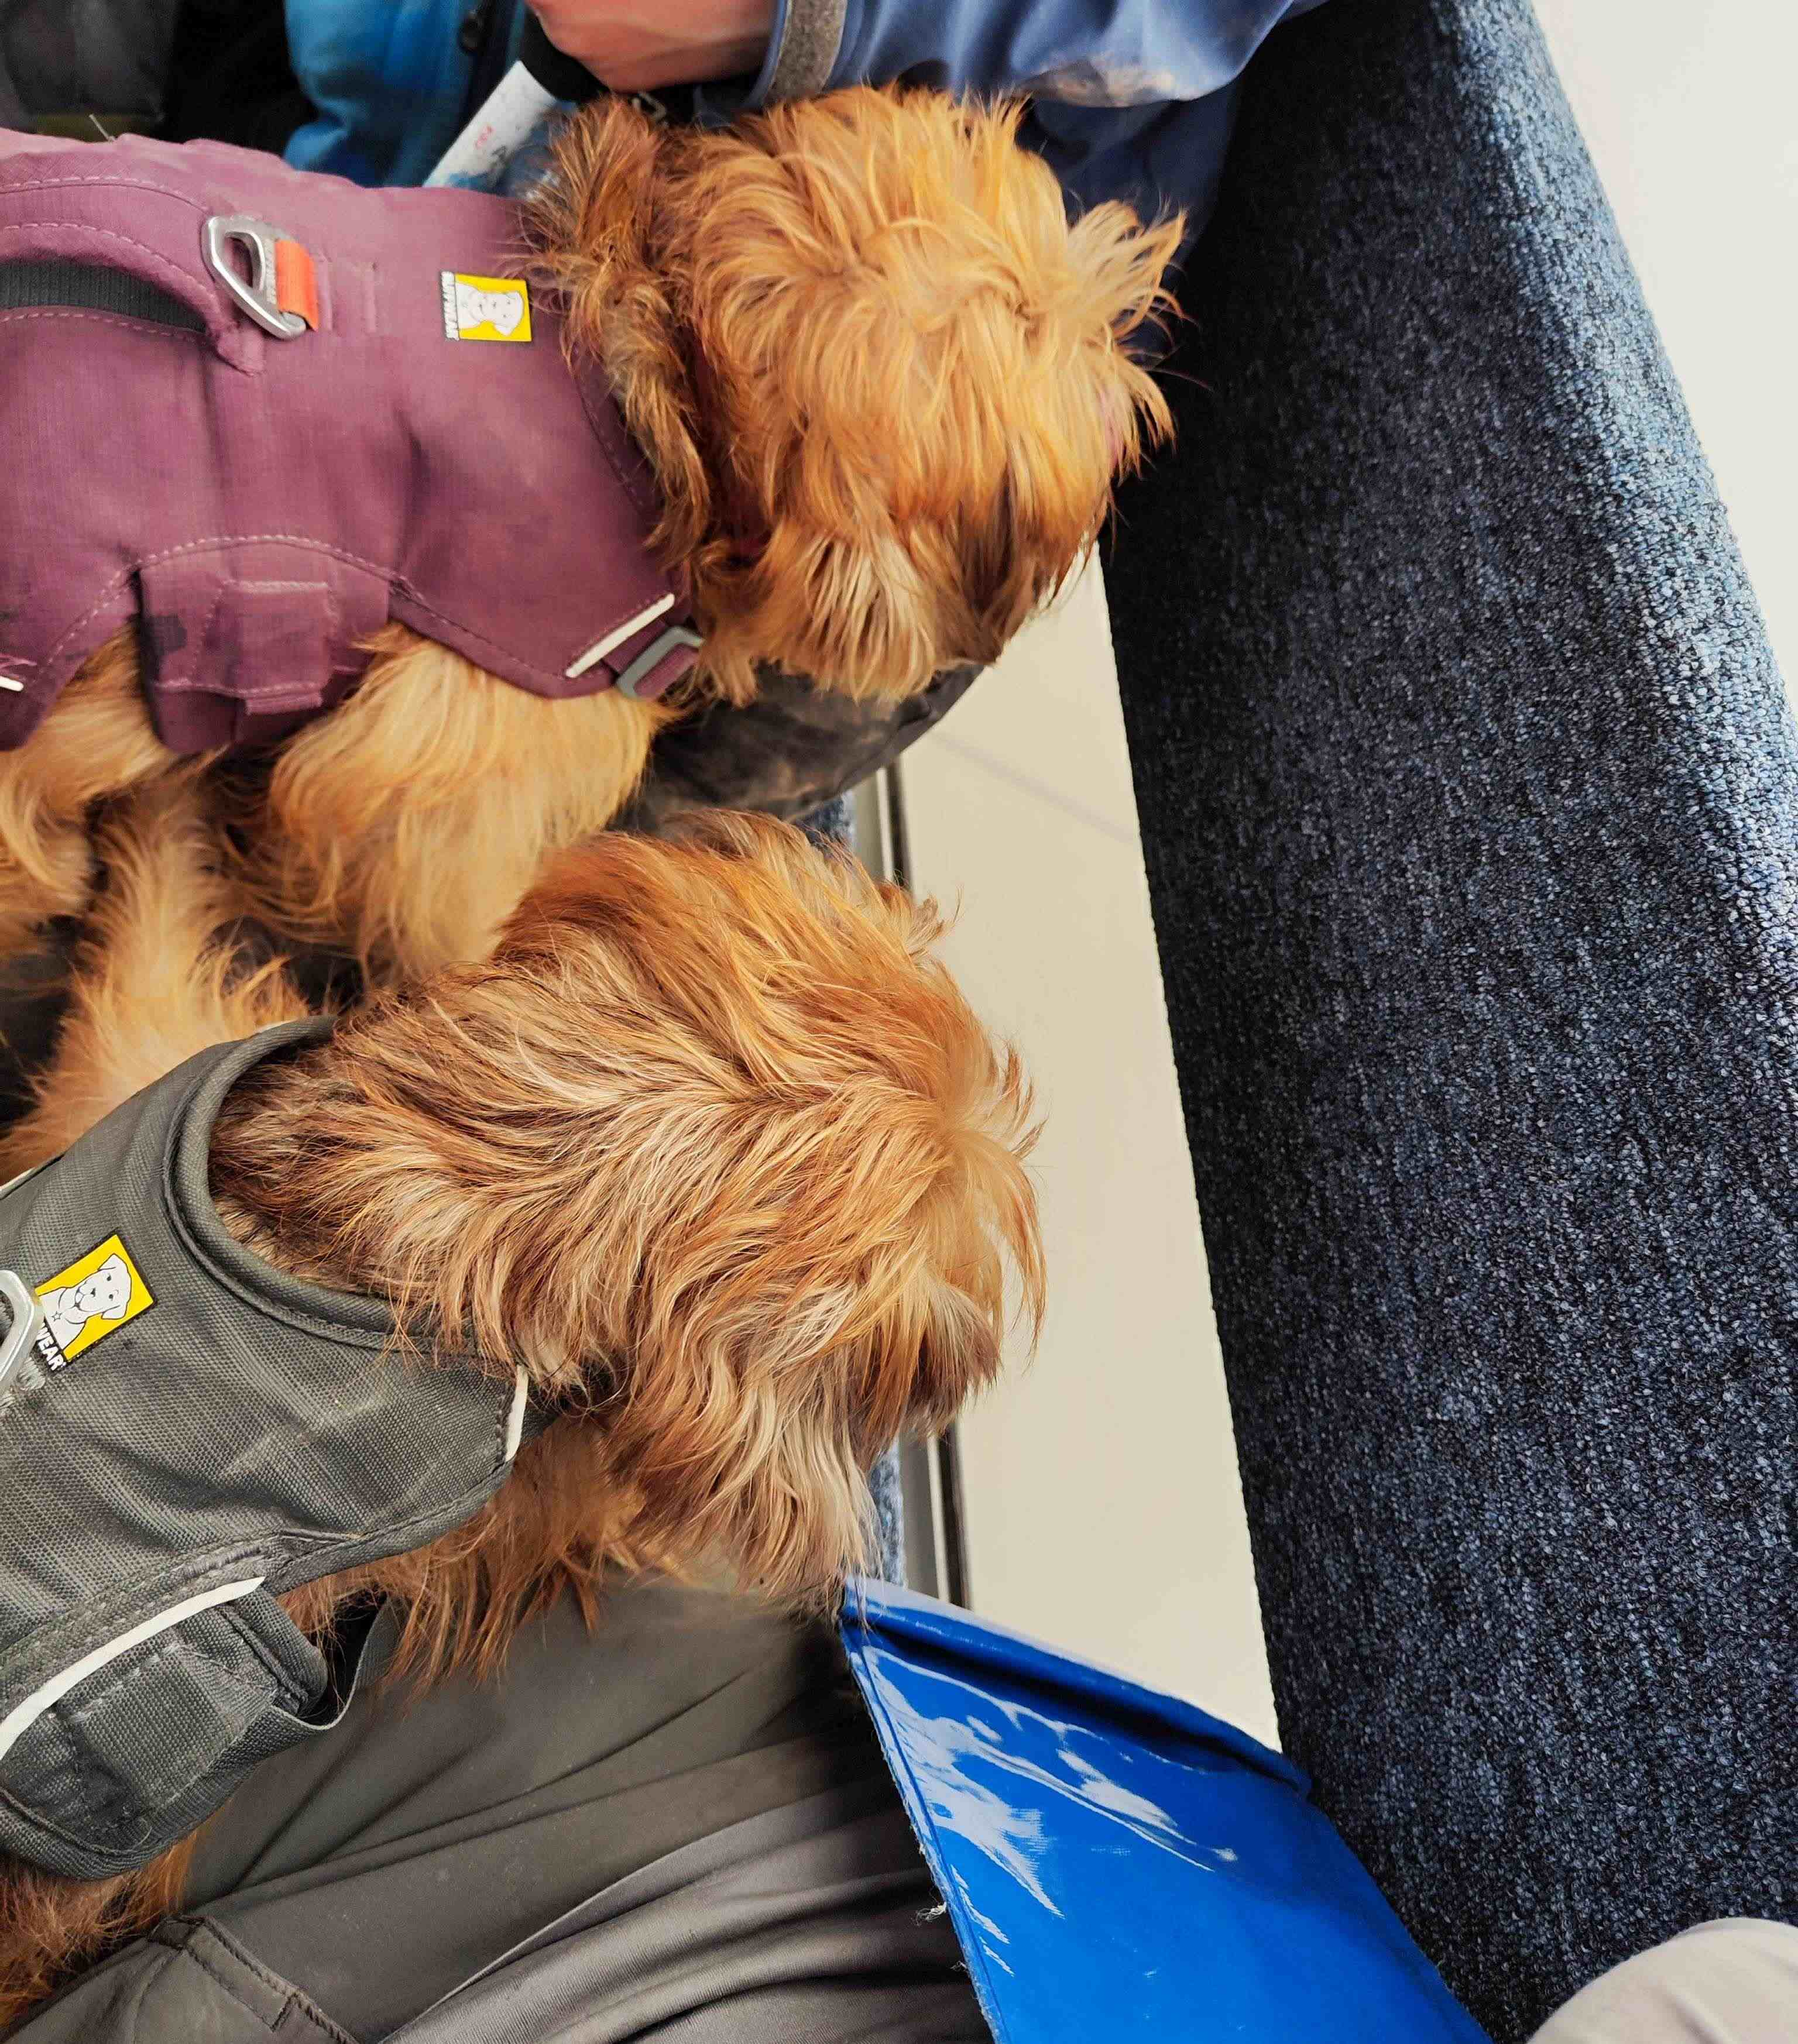
\includegraphics[width=0.35\linewidth]{../pics/IMG_20240830_170232.jpg}
	\caption{Собачки постигают новый для себя вид транспорта}
	\label{fig:IMG_20240830_170232.jpg}
\end{figure}

Спустившись в поляну Азау, оплатили безбилетный проезд в закрытой, но приоткрывшейся специально для нас кассе. С нас взяли стоимость спуска с самой верхней станции канатки~--- 1200~\faRub~с человека. Сообщили в МКК, МЧС и координатору о завершении машрута. На этом горная часть нашего путешествия завершилась.

\begin{figure}[h!]
	\centering
	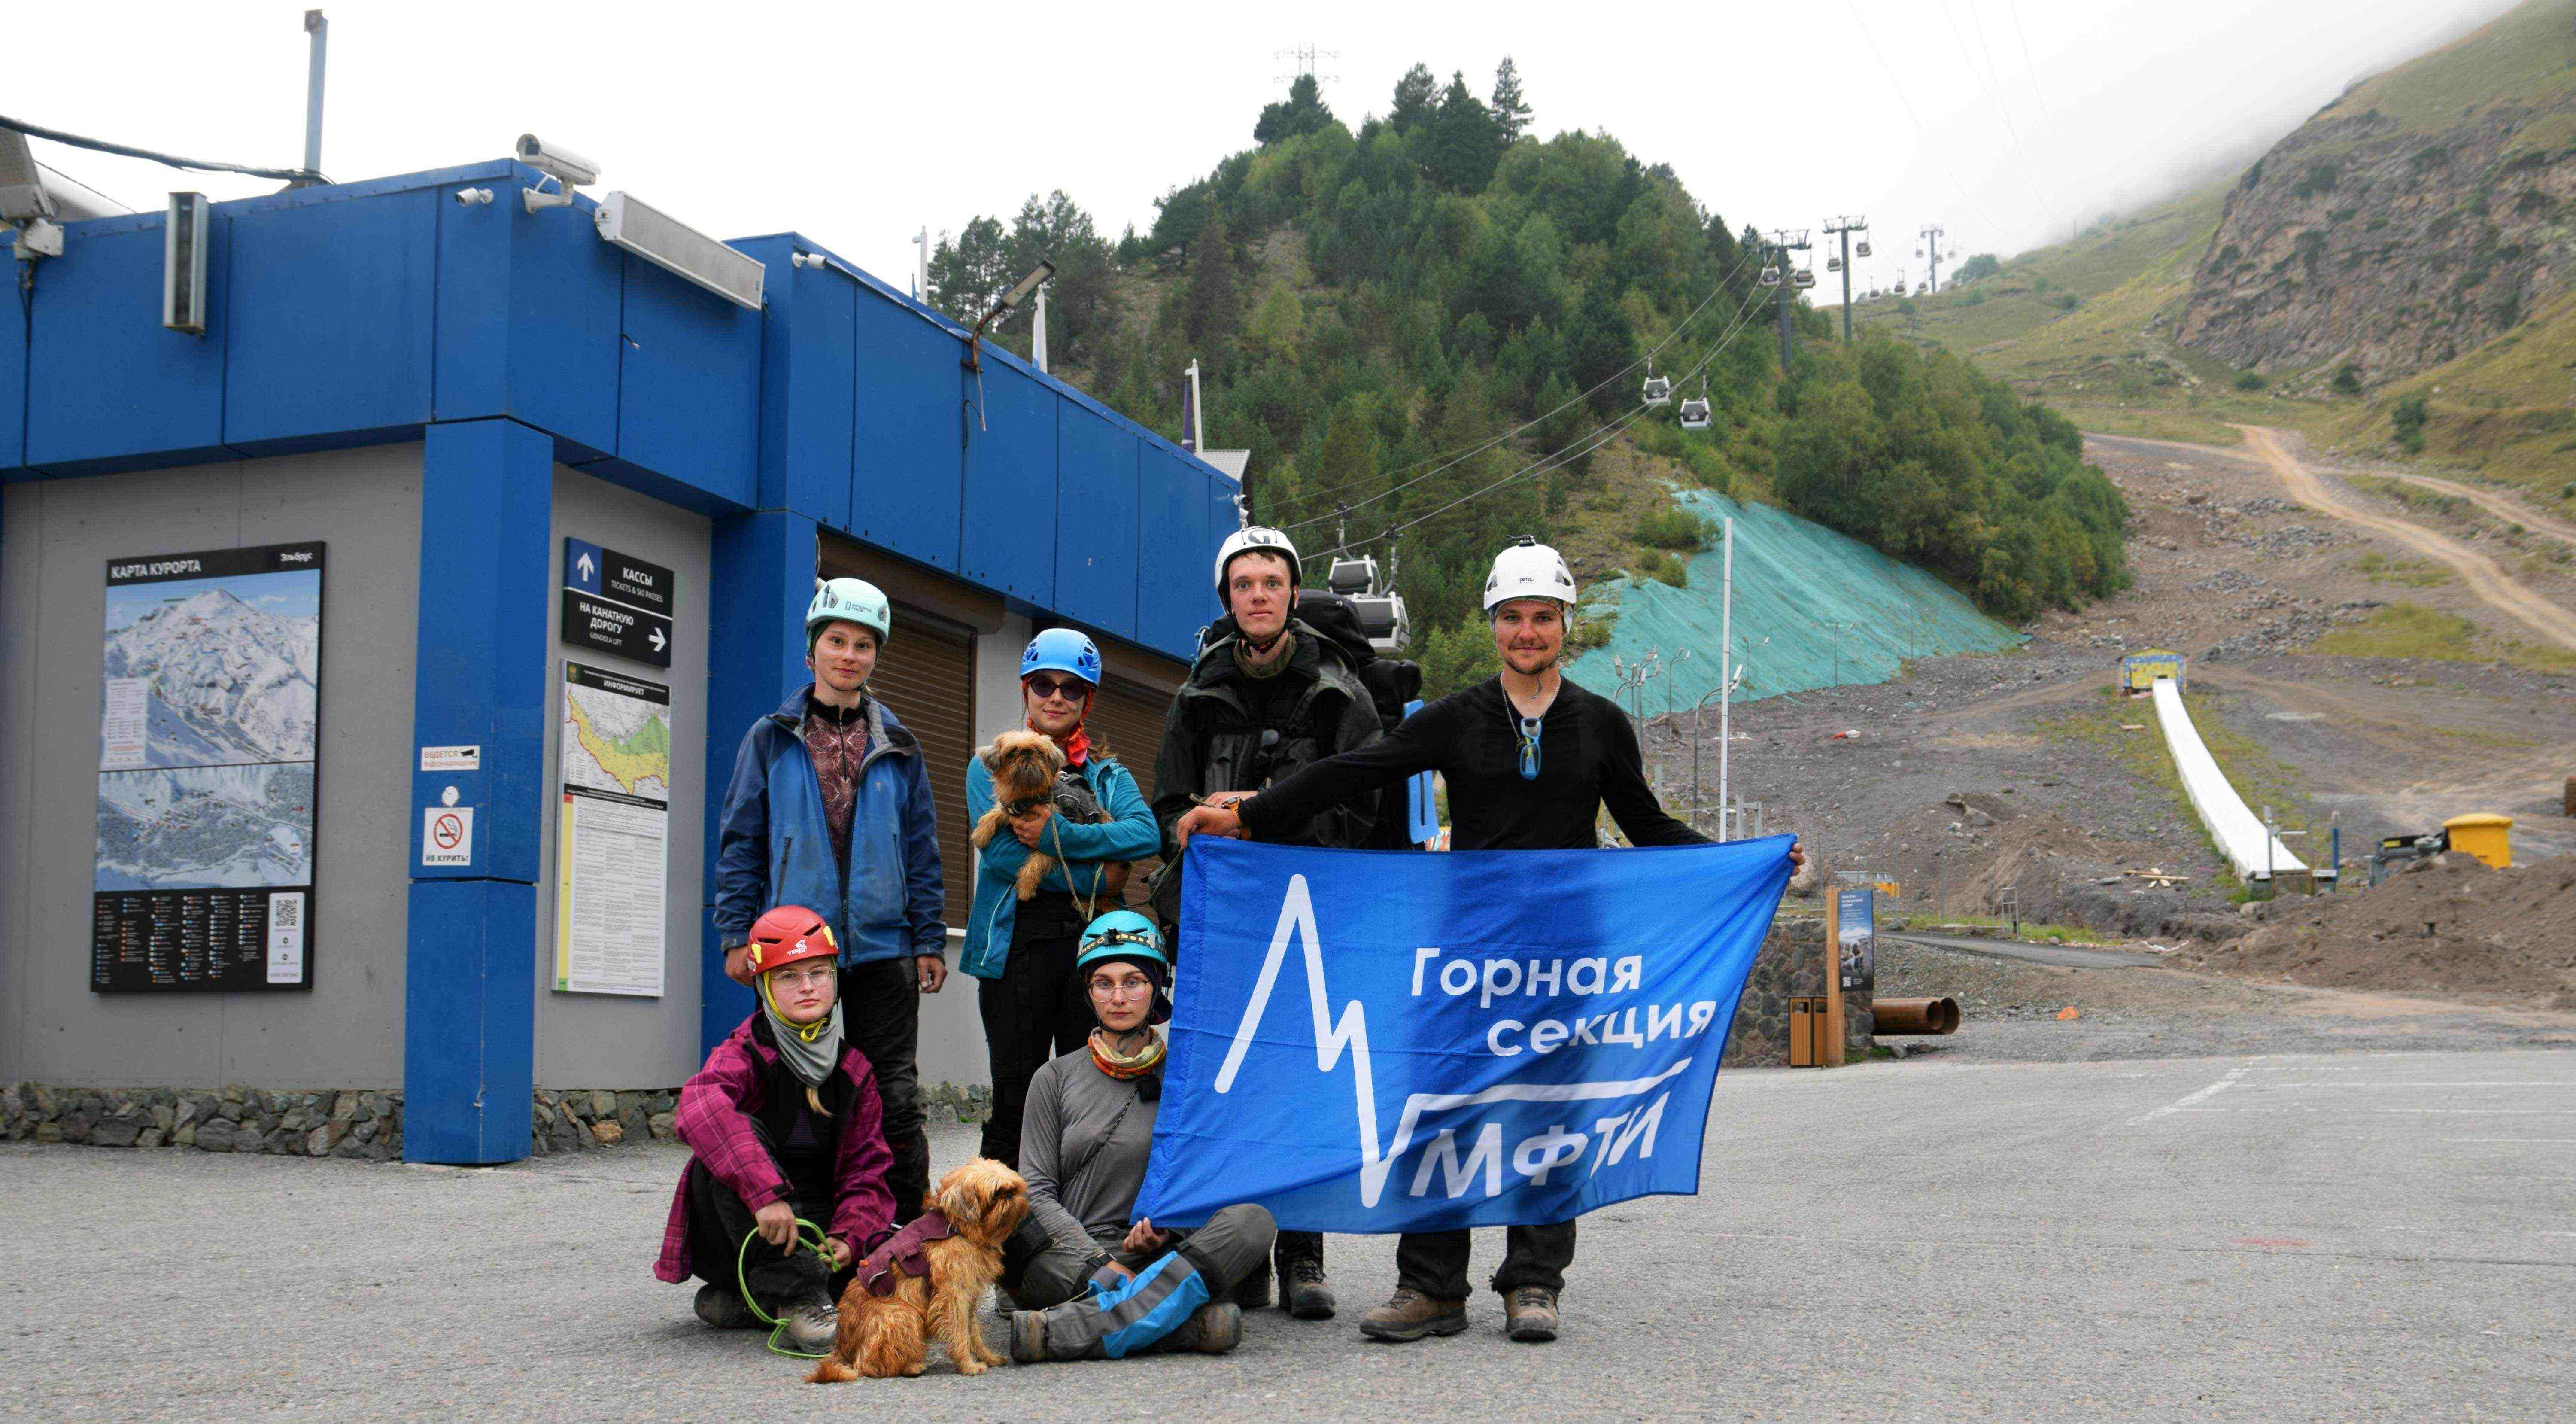
\includegraphics[width=0.7\linewidth]{../pics/group_finish.jpg}
	\caption{Конец путешествия, поляна Азау}
	\label{fig:group_finish}
\end{figure}

Остаток времени до прибытия трансфера провели в одной из кафешек поляны Азау.
В 20:00 нас встретил микроавтобус и повёз до железнодородного вокзала Минеральных Вод, где мы встретились с участниками, покинувшими нас в Хурзуке. Как только сели в автобус, начались дождь с грозой и градом, которыми пугал нас наш координатор, сообщая прогноз погоды. После полуночи загрузились в поезд и отправились домой!


\begin{table}[h!]
	\centering
	\begin{tabular}{|c|c|c|c|c|c|} 
		\hline 
		Этап & ЧХВ \\ 	
		\hline 
		Подход от слияния рек к каньону реки Уллукам		& 03:02\\
		Подъём по крутому травянистому склону до& 01:06 \\ выполаживания 
		Подход к месту ночёвки & 00:40 \\
		Подъём на седловину перевала Хотютау & 02:38\\
		Спуск с седловины до ледовых полей& 00:25\\
		Спуск по леднику до срединной морены & 01:50\\
		Обход зоны трещин, подход к озеру Эльбрусское& 01:00\\
		Спуск до ст. Кругозор & 00:40 \\
			
		\hline
		\textsc{Полное время подъёма на перевал  }& 07:26\\
		\textsc{Полное время спуска с перевала }& 03:55 \\
		\textsc{Полное время прохождения перевала }& 11:21 \\
		\hline
	\end{tabular}
	\caption{Расклад времени, пер. Хотютау}
\end{table}

\paragraph{Выводы и рекомендации:} пер. Хотютау в конце августа соответствует категории трудности 1А, т.к. ледник Большой Азау открыт. Прохождение перевала позволяет группе получить массу впечатлений от передвижения по ледовым полям, затяжным осыпным склонам, от потрясающих видов на Эльбрус, ГКХ, горные районы Карачаево-Черкессии и Кабардино-Балкарии. Настоятельно рекомендуется в качестве завершающего перевала в новичковых походах.


\clearpage